\documentclass[11pt, a4paper, twoside, openright]{article}

% Algorithms
	%\usepackage{algpseudocode}
	%\usepackage{algorithm}

% Babel
\usepackage[english]{babel}

% Code writing
	%\usepackage[procnames]{listings}

% Font
\usepackage[utf8]{inputenc}
\usepackage[T1]{fontenc}
\usepackage{amssymb,amsmath,amsthm,amsfonts}
\usepackage{eucal}
\usepackage{textcomp}

% Footnote


% Hyperref
\usepackage[hyphens]{url}
\usepackage{cite}
\usepackage{hyperref}
\usepackage{nameref}
\usepackage{url}
% Images
\usepackage[pdftex]{graphicx}
	%\usepackage{subfigure}
\usepackage{subfig}
\usepackage{eso-pic}
\usepackage{caption}
\usepackage{wrapfig}
\usepackage{float}

% List
\usepackage{enumerate}

% SI units
\usepackage{siunitx}

% Standalone
\usepackage[subpreambles=true]{standalone}
\usepackage{import}

% Tables
\usepackage{tabularx}
\usepackage{booktabs}
\usepackage{multirow}

% TiKz and graphs
\usepackage{pgf,tikz,pgfplots}
% \usepackage{gnuplottex}
\usepackage{bm}
\usepackage{relsize}
%\usepackage[compat=1.1.0]{tikz-feynman}
\usepackage{circuitikz}

% Typeset
%\usepackage[top=2cm,bottom=2cm,left=2cm,right=2cm]{geometry}
\usepackage[top=2cm,bottom=2cm,left=2cm,right=2cm]{geometry}
\usepackage{fancyhdr}
\usepackage{indentfirst}
\usepackage{titlesec}
\usepackage{setspace}
\usepackage{xspace}
% \usepackage{parskip}  % Elimina il separatore a inizio paragrafo
\usepackage{afterpage}
\usepackage{comment}

%Python
\usepackage{xcolor}
\usepackage{listings}
\usepackage{framed}

%Per scrivere matrice identità
\usepackage{bbold}
%Per semplificazione formule
\usepackage{cancel}

%Evidenziare formule
\usepackage{empheq}
	%oppure
	%\usepackage{xcolor}
\usepackage{soul}

%Evidenziare testo con mdframed
\usepackage{mdframed}

%Note a margine
\usepackage{marginnote}

%Display data
\usepackage{datetime}

%Physics
\usepackage{physics}

%Geometry
%\newgeometry{inner=20mm,
%            outer=49mm,% = marginparsep + marginparwidth
%                       %   + 5mm (between marginpar and page border)
%            top=20mm,
%            bottom=25mm,
%            marginparsep=6mm,
%            marginparwidth=30mm}
%\makeatletter
%\renewcommand{\@marginparreset}{%
%  \reset@font\small
%  \raggedright
%  \slshape
%  \@setminipage
%}
%\makeatother

%Atom Latex
%\pgfplotsset{compat=1.15}

%%
\captionsetup[table]{font=small,labelfont={bf},skip=10pt}
\captionsetup[figure]{font=small,labelfont={bf},skip=10pt}

%intestazione pagina
%\pagestyle{fancy}
%\fancyhf{}
%\fancyhead[RE]{\ifnum\value{chapter}>0\nouppercase{\leftmark}\fi}
%\fancyhead[LE]{\small\textbf{\thepage}}
%\fancyhead[LO]{\nouppercase{\rightmark}}
%\fancyhead[RO]{\small\textbf{\thepage}}

%link ipertestuale per indice
\hypersetup{
	colorlinks=false,
	linkcolor=black,
	filecolor=blue,
	citecolor = blue,
	urlcolor=blue,
	}

%%%%%indent%%%
\setlength{\parindent}{15pt}
\setlength{\parskip}{0pt}


%boh
%\renewcommand{\chaptermark}[1]{%
% \markboth{\MakeUppercase{%
% \chaptername}\ \thechapter.%
% \ #1}{}}


 %Python in latex
 \definecolor{codegreen}{rgb}{0,0.6,0}
\definecolor{codegray}{rgb}{0.5,0.5,0.5}
\definecolor{codepurple}{rgb}{0.58,0,0.82}
\definecolor{backcolour}{rgb}{0.95,0.95,0.92}
\definecolor{commentcolour}{rgb}{0.43,0.63,0.65}

\definecolor{shadecolor}{rgb}{0.93, 0.93, 0.93}
\definecolor{darkgreen}{rgb}{0.0, 0.5, 0.0}
\definecolor{darkred}{rgb}{0.8, 0.0, 0.0}
\definecolor{violet}{rgb}{0.55, 0.0, 0.55}

\lstdefinestyle{mystyle}{ %Stile python code
    backgroundcolor=\color{shadecolor},
    commentstyle=\color{commentcolour},
    keywordstyle=\color{darkgreen},
    numberstyle=\tiny\color{codegray},
    stringstyle=\color{darkred},
    basicstyle=\footnotesize\ttfamily,
    breakatwhitespace=false,
    breaklines=true,
    captionpos=b,
    keepspaces=true,
    numbers=left,
    numbersep=5pt,
    showspaces=false,
    showstringspaces=false,
    showtabs=false,
    tabsize=2
}

\lstset{
    style=mystyle
}

%VHDL in latex
\usepackage{beramono}
\lstdefinelanguage{VHDL}{
   morekeywords={
     library,use,all,entity,is,port,in,out,end,architecture,of,
     begin,and
   },
   morecomment=[l]--
}
\colorlet{keyword}{blue!100!black!80}
\colorlet{comment}{green!90!black!90}
\lstdefinestyle{vhdl}{
   language     = VHDL,
   basicstyle   = \ttfamily\footnotesize,
   keywordstyle = \color{keyword}\bfseries,
   commentstyle = \color{comment}
}


% Derivatives
\renewcommand{\d}[0]{\mathrm{d}}
\newcommand{\dev}[2]{\displaystyle \frac{\d #1}{\d #2}}
\newcommand{\pdev}[2]{\displaystyle \frac{\partial #1}{\partial #2}}
\newcommand{\ndev}[3]{\displaystyle \frac{\d^{#3} #1}{\d #2^{#3} } }
\newcommand{\npdev}[3]{\displaystyle \frac{\partial^{#3} #1}{\partial #2^{#3} } }


%% Norms
\newcommand{\absvec}[1]{| \vec{#1} |}
\newcommand{\normvec}[1]{|\!| \vec{#1} |\!|}

\newcommand{\vmed}[1]{\left \langle #1 \right \rangle}
\newcommand{\vmedvec}[1]{\langle #1 \rangle}
\newcommand{\R}[0]{\mathbb{R}}
\renewcommand{\H}[0]{\operatorname{H}}

%Evidenziare formule
\newcommand{\mathcolorbox}[2]{\colorbox{#1}{$\displaystyle #2$}}
\newcommand{\hlfancy}[2]{\sethlcolor{#1}\hl{#2}}

%Theorem
\newtheorem{theorem}{Theorem}[section]
\newtheorem{corollary}{Corollary}[theorem]
\newtheorem{lemma}[theorem]{Lemma}
\newtheorem{proposition}[theorem]{Proposition}

\theoremstyle{definition}
\newtheorem{definition}{Definition}%[section]


%%%%%%%%%%%%%%%%%%%%Exercise and example%%%%%%%%%%%%%%%%%
\usepackage[many,most,theorems]{tcolorbox}


\newtcbtheorem{exercise}{Exercise}{ % frame stuff
    boxrule = 1pt,
    breakable,
    enhanced,
    frame empty,
    interior style= {blue!6},
    %interior empty,
    colframe=black,
    borderline ={1pt}{0pt}{black},
    left=0.2cm,
    % title stuff
    attach boxed title to top left={yshift=-2mm,xshift=0mm},
    coltitle=black,
    fonttitle=\bfseries,
    colbacktitle=white,
    boxed title style={boxrule=1pt,sharp corners}}{exercise} 

\newtcbtheorem{example}{Example}{ % frame stuff
    boxrule = 1pt,
    enhanced,
    frame empty,
    interior style= {green!6},%{left color=yellow!70,right color=green!70},
    %interior empty,
    colframe=black,
    borderline ={1pt}{0pt}{black},
    breakable,
    left=0.2cm,
    % title stuff
    attach boxed title to top left={yshift=-2mm,xshift=0mm},
    coltitle=black,
    fonttitle=\bfseries,
    colbacktitle=white,
    boxed title style={boxrule=1pt,sharp corners}}{example}
  
%\newtheorem{exercise}{Exercise}
%\newtheorem{example}{Example}

%%%%%%%%%%%%%%%%%%%%%%%%%%%%%%%%%%%

\theoremstyle{remark}
\newtheorem*{remark}{Remark}
\newtheorem{observation}{Observation}
%Evidenziare testo
\newtheorem*{solution}{Solution}

\newcommand\mybox[1]{%
  \fbox{\begin{minipage}{0.9\textwidth}#1\end{minipage}}}

  %Spiegazioni/verifiche
\newenvironment{greenbox}{\begin{mdframed}[hidealllines=true,backgroundcolor=green!20,innerleftmargin=3pt,innerrightmargin=3pt,innertopmargin=3pt,innerbottommargin=3pt]}{\end{mdframed}}

\newenvironment{bluebox}{\begin{mdframed}[hidealllines=true,backgroundcolor=blue!10,innerleftmargin=3pt,innerrightmargin=3pt,innertopmargin=3pt,innerbottommargin=3pt]}{\end{mdframed}}

\newenvironment{yellowbox}{\begin{mdframed}[hidealllines=true,backgroundcolor=yellow!20,innerleftmargin=3pt,innerrightmargin=3pt,innertopmargin=3pt,innerbottommargin=3pt]}{\end{mdframed}}

\newenvironment{redbox}{\begin{mdframed}[hidealllines=true,backgroundcolor=red!20,innerleftmargin=3pt,innerrightmargin=3pt,innertopmargin=3pt,innerbottommargin=3pt]}{\end{mdframed}}

\newenvironment{orangebox}{\begin{mdframed}[hidealllines=true,backgroundcolor=orange!20,innerleftmargin=3pt,innerrightmargin=3pt,innertopmargin=3pt,innerbottommargin=3pt]}{\end{mdframed}}

%emph equation
\newcommand*\myyellowbox[1]{%
  \colorbox{yellow!40}{\hspace{1em}#1\hspace{1em}}}

\newcommand*\mygreenbox[1]{%
  \colorbox{green!20}{\hspace{1em}#1\hspace{1em}}}
  
  
  
  
  


\begin{document}

\title{\textbf{Homework 1}}

\author{Alice Pagano \\ 1236916}

\maketitle

\section{Total-number operator and Hamiltonian commute}

Show, using the formalism of the second quantization, that, for both \textbf{bosons} and \textbf{fermions} the total-number operator and the Hamiltonian operator commute: \( \pmb{[N,H]=0} \).
\begin{proof}
Let us consider the \textbf{field operators}:
\begin{equation}
  \begin{cases}
 \hat{\psi }_ \alpha  (\va{x}) \equiv  \sum_{\va{k}}^{} \varphi _{\va{k}, \alpha } (\va{x}) c_{\va{k}, \alpha }  \\
\hat{\psi }_ \alpha ^\dag   (\va{x}) \equiv  \sum_{\va{k}}^{} \varphi _{\va{k}, \alpha } ^\dag  (\va{x}) c_{\va{k}, \alpha } ^\dag
\end{cases}
\end{equation}
The field operators satisfy simple \emph{commutation} or \emph{anticommutation} relations depending on the statistics:
\begin{equation}
  \begin{cases}
    [\hat{\psi }_ \alpha (\va{x}), \hat{\psi }_ \beta ^\dag (\va{x}')  ]_\pm = \delta _{\alpha \beta } \delta (\va{x}-\va{x}') \\
   [\hat{\psi }_ \alpha (\va{x}), \hat{\psi }_ \beta (\va{x}')  ]_\pm = 0 \\
   [\hat{\psi }_ \alpha ^\dag (\va{x}), \hat{\psi }_ \beta ^\dag (\va{x}')  ]_\pm = 0
  \end{cases}
\end{equation}
where the upper (lower) sign refers to bosons (fermions).

In second quantization and in terms of these field operators:
\begin{itemize}
\item the \textbf{total-number operator} can be written as:
\begin{equation}
  \hat{N} = \int_{}^{} \dd[3]{\va{x}''} n(\va{x}'')
= \sum_{i}^{} c_i ^\dag c_i = \sum_{i}^{} \hat{n}_i =
\int_{}^{} \dd[3]{\va{x}''} \hat{\psi }^\dag (\va{x}'') \hat{\psi }(\va{x}'')
\end{equation}
\item the \textbf{Hamiltonian} operator can be written as:
\begin{equation}
  \hat{H} =
  \underbrace{
   \int_{}^{} \dd[3]{\va{x}} \hat{\psi } ^\dag  (\va{x}) T (\va{x}) \hat{\psi }(\va{x})
   }_{\equiv \hat{T} }
+
\underbrace{
 \frac{1}{2}  \int_{}^{} \dd[3]{\va{x}}
\int_{}^{} \dd[3]{\va{x}'} \hat{\psi } ^\dag (\va{x})
\hat{\psi } ^\dag (\va{x}') V (\va{x},\va{x}') \hat{\psi } (\va{x}') \hat{\psi } (\va{x})
 }_{\equiv \hat{V} }
\end{equation}
\end{itemize}

\subsection*{Case: fermions}
Let us consider separately the commutator between the kinetic and the potential terms:
\begin{equation*}
  [\hat{N}, \hat{H}  ] = [\hat{N}, \hat{T}  ] + [\hat{N}, \hat{V}  ]
\end{equation*}

\subsubsection*{Kinetic term}
\begin{equation*}
\begin{split}
  [\hat{N},\hat{T}  ]&= \hat{N}\hat{T} - \hat{T}\hat{N} \\
  &=  \int_{}^{} \dd[3]{\va{x}''} \hat{\psi }^\dag (\va{x}'') \hat{\psi }(\va{x}'')
      \int_{}^{} \dd[3]{\va{x}} \hat{\psi } ^\dag  (\va{x}) T (\va{x}) \hat{\psi }(\va{x})
      -
      \int_{}^{} \dd[3]{\va{x}} \hat{\psi } ^\dag  (\va{x}) T (\va{x}) \hat{\psi }(\va{x})
      \int_{}^{} \dd[3]{\va{x}''} \hat{\psi }^\dag (\va{x}'') \hat{\psi }(\va{x}'') \\
  &= \int_{}^{} \int_{}^{} \dd[3]{\va{x}''} \dd[3]{\va{x}}  \hat{\psi }^\dag (\va{x}'') \mathcolorbox{green!20}{ \hat{\psi }(\va{x}'') \hat{\psi } ^\dag  (\va{x}) }  T (\va{x}) \hat{\psi }(\va{x})
      - \int_{}^{} \int_{}^{} \dd[3]{\va{x}} \dd[3]{\va{x}''} \hat{\psi } ^\dag  (\va{x}) T (\va{x}) \mathcolorbox{green!20}{ \hat{\psi }(\va{x}) \hat{\psi }^\dag (\va{x}'') } \hat{\psi }(\va{x}'')
\end{split}
\end{equation*}
Now, using the relation:
\begin{equation}
\begin{split}
  \{ \hat{\psi } (\va{x}''), \hat{\psi }^\dag (\va{x}) \} &=   \hat{\psi } (\va{x}'') \hat{\psi }^\dag (\va{x}) +   \hat{\psi }^\dag (\va{x}) \hat{\psi } (\va{x}'') = \delta (\va{x}''-\va{x})  \\
  & \Rightarrow \hat{\psi } (\va{x}'') \hat{\psi }^\dag (\va{x}) = - \hat{\psi }^\dag (\va{x}) \hat{\psi } (\va{x}'') + \delta (\va{x}''-\va{x})
\end{split}
\label{eq:anticommutator}
\end{equation}
the green terms transform as:
\begin{equation*}
\begin{split}
  [\hat{N},\hat{T}  ] &=
      \int_{}^{} \int_{}^{} \dd[3]{\va{x}''} \dd[3]{\va{x}}  \hat{\psi }^\dag (\va{x}'') \mathcolorbox{green!20}{  \qty( - \hat{\psi }^\dag (\va{x}) \hat{\psi } (\va{x}'') )
      }   T (\va{x}) \hat{\psi }(\va{x})
      + \int_{}^{} \int_{}^{} \dd[3]{\va{x}''} \dd[3]{\va{x}}  \hat{\psi }^\dag (\va{x}'') \mathcolorbox{green!20}{  \qty( \delta (\va{x}''-\va{x}) )
      }   T (\va{x}) \hat{\psi }(\va{x})
      \\
      &-
      \int_{}^{} \int_{}^{} \dd[3]{\va{x}} \dd[3]{\va{x}''} \hat{\psi } ^\dag  (\va{x}) T (\va{x}) \mathcolorbox{green!20}{ \qty(- \hat{\psi }^\dag (\va{x}'') \hat{\psi } (\va{x})) } \hat{\psi }(\va{x}'')
      - \int_{}^{} \int_{}^{} \dd[3]{\va{x}} \dd[3]{\va{x}''} \hat{\psi } ^\dag  (\va{x}) T (\va{x}) \mathcolorbox{green!20}{  \qty( \delta (\va{x}''-\va{x}) ) } \hat{\psi }(\va{x}'') \\
      & \overset{(a)}{=}
      - \int_{}^{} \int_{}^{} \dd[3]{\va{x}''} \dd[3]{\va{x}}  \hat{\psi }^\dag (\va{x}'')  \hat{\psi }^\dag (\va{x}) T (\va{x}) \mathcolorbox{yellow!40}{\hat{\psi } (\va{x}'')}
       \hat{\psi }(\va{x})
      + \cancel{ \int_{}^{} \int_{}^{} \dd[3]{\va{x}} \dd[3]{\va{x}}  \hat{\psi }^\dag (\va{x}) T (\va{x}) \hat{\psi }(\va{x}) }
      \\
      &+
      \int_{}^{} \int_{}^{} \dd[3]{\va{x}} \dd[3]{\va{x}''} \hat{\psi } ^\dag  (\va{x})  \mathcolorbox{yellow!40}{ \hat{\psi }^\dag (\va{x}'') } T (\va{x})  \hat{\psi } (\va{x}) \hat{\psi }(\va{x}'')
      - \cancel{ \int_{}^{} \int_{}^{} \dd[3]{\va{x}} \dd[3]{\va{x}} \hat{\psi } ^\dag  (\va{x}) T (\va{x}) \hat{\psi }(\va{x}) }  \\
      & =
      - \int_{}^{} \int_{}^{} \dd[3]{\va{x}''} \dd[3]{\va{x}}  \hat{\psi }^\dag (\va{x}'')  \hat{\psi }^\dag (\va{x})
      T (\va{x}) \hat{\psi } (\va{x}'') \hat{\psi }(\va{x})
      +
      \int_{}^{} \int_{}^{} \dd[3]{\va{x}} \dd[3]{\va{x}''} \mathcolorbox{orange!40}{ \hat{\psi } ^\dag  (\va{x})   \hat{\psi }^\dag (\va{x}'') } T (\va{x})  \mathcolorbox{pink!40}{ \hat{\psi } (\va{x}) \hat{\psi }(\va{x}'') }
\end{split}
\end{equation*}
where in \( (a) \) we have interchanged the yellow terms with the kinetic term \( T(\va{x}) \), since it acts only in \( \va{x} \).
Then, using the following commutation rules in the orange and pink terms:
\begin{equation}
  \begin{cases}
   \{ \hat{\psi } ^\dag (\va{x}), \hat{\psi }^\dag (\va{x}'') \}=0 & \Rightarrow  \hat{\psi } ^\dag (\va{x}) \hat{\psi }^\dag (\va{x}'') = - \hat{\psi }^\dag (\va{x}'') \hat{\psi } ^\dag (\va{x}) \\
   \{ \hat{\psi }  (\va{x}), \hat{\psi }(\va{x}'') \}=0 & \Rightarrow  \hat{\psi }  (\va{x}) \hat{\psi } (\va{x}'') = - \hat{\psi } (\va{x}'') \hat{\psi } (\va{x})
  \end{cases}
  \label{eq:anticommutator_0}
\end{equation}
we obtain:
\begin{equation*}
\begin{split}
  [\hat{N},\hat{T}  ] &=
    \cancel{- \int_{}^{} \int_{}^{} \dd[3]{\va{x}''} \dd[3]{\va{x}}  \hat{\psi }^\dag (\va{x}'')  \hat{\psi }^\dag (\va{x})
    T (\va{x}) \hat{\psi } (\va{x}'') \hat{\psi }(\va{x})}
    +
    \cancel{\int_{}^{} \int_{}^{} \dd[3]{\va{x}} \dd[3]{\va{x}''} \mathcolorbox{orange!40}{    \hat{\psi }^\dag (\va{x}'') \hat{\psi } ^\dag  (\va{x}) } T (\va{x})  \mathcolorbox{pink!40}{  \hat{\psi }(\va{x}'') \hat{\psi } (\va{x}) }} \\
    &= 0
\end{split}
\end{equation*}

\subsubsection*{Potential term}
\begin{equation*}
\begin{split}
[\hat{N},\hat{V}  ]  =&  \hat{N}\hat{V} - \hat{V}\hat{N}     \\
    =& \int_{}^{} \dd[3]{\va{x}''} \hat{\psi }^\dag (\va{x}'') \hat{\psi }(\va{x}'') \frac{1}{2}  \int_{}^{} \dd[3]{\va{x}}
     \int_{}^{} \dd[3]{\va{x}'} \hat{\psi } ^\dag (\va{x})
     \hat{\psi } ^\dag (\va{x}') V (\va{x},\va{x}') \hat{\psi } (\va{x}') \hat{\psi } (\va{x}) \\
     &-
     \frac{1}{2}  \int_{}^{} \dd[3]{\va{x}}
      \int_{}^{} \dd[3]{\va{x}'} \hat{\psi } ^\dag (\va{x})
      \hat{\psi } ^\dag (\va{x}') V (\va{x},\va{x}') \hat{\psi } (\va{x}') \hat{\psi } (\va{x})
      \int_{}^{} \dd[3]{\va{x}''} \hat{\psi }^\dag (\va{x}'') \hat{\psi }(\va{x}'') \\
    =&
    \frac{1}{2} \int_{}^{} \int_{}^{} \int_{}^{} \dd[3]{\va{x}''} \dd[3]{\va{x}}  \dd[3]{\va{x}'}
    \hat{\psi }^\dag (\va{x}'') \mathcolorbox{green!20}{ \hat{\psi }(\va{x}'') \hat{\psi } ^\dag (\va{x}) }
    \hat{\psi } ^\dag (\va{x}') V (\va{x},\va{x}') \hat{\psi } (\va{x}') \hat{\psi } (\va{x}) \\
    &- \frac{1}{2} \int_{}^{} \int_{}^{} \int_{}^{} \dd[3]{\va{x}} \dd[3]{\va{x}'} \dd[3]{\va{x}''}
    \hat{\psi } ^\dag (\va{x})
    \hat{\psi } ^\dag (\va{x}') V (\va{x},\va{x}') \hat{\psi } (\va{x}') \mathcolorbox{green!20}{\hat{\psi } (\va{x}) \hat{\psi }^\dag (\va{x}'')} \hat{\psi }(\va{x}'') \\
     \overset{\eqref{eq:anticommutator}}{=} &
    \frac{1}{2} \int_{}^{} \int_{}^{} \int_{}^{} \dd[3]{\va{x}''} \dd[3]{\va{x}}  \dd[3]{\va{x}'}
    \hat{\psi }^\dag (\va{x}'') \mathcolorbox{green!20}{ \qty(-  \hat{\psi } ^\dag (\va{x}) \hat{\psi }(\va{x}'')  ) }
    \hat{\psi } ^\dag (\va{x}') V (\va{x},\va{x}') \hat{\psi } (\va{x}') \hat{\psi } (\va{x}) \\
    &+
    \frac{1}{2} \int_{}^{} \int_{}^{} \int_{}^{} \dd[3]{\va{x}''} \dd[3]{\va{x}}  \dd[3]{\va{x}'}
    \hat{\psi }^\dag (\va{x}'') \mathcolorbox{green!20}{ \qty(\delta (\va{x}''-\va{x}) ) }
    \hat{\psi } ^\dag (\va{x}') V (\va{x},\va{x}') \hat{\psi } (\va{x}') \hat{\psi } (\va{x}) \\
    &-
    \frac{1}{2} \int_{}^{} \int_{}^{} \int_{}^{} \dd[3]{\va{x}} \dd[3]{\va{x}'} \dd[3]{\va{x}''}
    \hat{\psi } ^\dag (\va{x})
    \hat{\psi } ^\dag (\va{x}') V (\va{x},\va{x}') \hat{\psi } (\va{x}') \mathcolorbox{green!20}{ \qty(-   \hat{\psi }^\dag (\va{x}'') \hat{\psi } (\va{x})  )} \hat{\psi }(\va{x}'') \\
    &-
    \frac{1}{2} \int_{}^{} \int_{}^{} \int_{}^{} \dd[3]{\va{x}} \dd[3]{\va{x}'} \dd[3]{\va{x}''}
    \hat{\psi } ^\dag (\va{x})
    \hat{\psi } ^\dag (\va{x}') V (\va{x},\va{x}') \hat{\psi } (\va{x}') \mathcolorbox{green!20}{ \qty( \delta (\va{x}''-\va{x}))} \hat{\psi }(\va{x}'')
\end{split}
\end{equation*}
Thus, by exploiting the \( \delta (\va{x}''-\va{x}) \):
\begin{equation*}
\begin{split}
  [\hat{N},\hat{V}  ] =&
      - \frac{1}{2} \int_{}^{} \int_{}^{} \int_{}^{} \dd[3]{\va{x}''} \dd[3]{\va{x}}  \dd[3]{\va{x}'}
      \hat{\psi }^\dag (\va{x}'')   \hat{\psi } ^\dag (\va{x}) \mathcolorbox{yellow!40}{\hat{\psi }(\va{x}'')
      \hat{\psi } ^\dag (\va{x}')} V (\va{x},\va{x}') \hat{\psi } (\va{x}') \hat{\psi } (\va{x}) \\
      &+
      \bcancel{
      \frac{1}{2} \int_{}^{} \int_{}^{} \int_{}^{} \dd[3]{\va{x}} \dd[3]{\va{x}}  \dd[3]{\va{x}'}
      \hat{\psi }^\dag (\va{x})
      \hat{\psi } ^\dag (\va{x}') V (\va{x},\va{x}') \hat{\psi } (\va{x}') \hat{\psi } (\va{x})
      } \\
      &+
      \frac{1}{2} \int_{}^{} \int_{}^{} \int_{}^{} \dd[3]{\va{x}} \dd[3]{\va{x}'} \dd[3]{\va{x}''}
      \hat{\psi } ^\dag (\va{x})
      \hat{\psi } ^\dag (\va{x}') V (\va{x},\va{x}') \mathcolorbox{yellow!40}{\hat{\psi } (\va{x}')   \hat{\psi }^\dag (\va{x}'') } \hat{\psi } (\va{x}) \hat{\psi }(\va{x}'') \\
      &-
      \bcancel{
      \frac{1}{2} \int_{}^{} \int_{}^{} \int_{}^{} \dd[3]{\va{x}} \dd[3]{\va{x}'} \dd[3]{\va{x}}
      \hat{\psi } ^\dag (\va{x})
      \hat{\psi } ^\dag (\va{x}') V (\va{x},\va{x}') \hat{\psi } (\va{x}')  \hat{\psi }(\va{x})
      } \\
      \overset{\eqref{eq:anticommutator}}{=} &
      - \frac{1}{2} \int_{}^{} \int_{}^{} \int_{}^{} \dd[3]{\va{x}''} \dd[3]{\va{x}}  \dd[3]{\va{x}'}
      \hat{\psi }^\dag (\va{x}'')   \hat{\psi } ^\dag (\va{x}) \mathcolorbox{yellow!40}{ \qty( - \hat{\psi } ^\dag (\va{x}')  \hat{\psi }(\va{x}'') )} V (\va{x},\va{x}') \hat{\psi } (\va{x}') \hat{\psi } (\va{x}) \\
      &-
      \frac{1}{2} \int_{}^{} \int_{}^{} \int_{}^{} \dd[3]{\va{x}''} \dd[3]{\va{x}}  \dd[3]{\va{x}'}
      \hat{\psi }^\dag (\va{x}'')   \hat{\psi } ^\dag (\va{x}) \mathcolorbox{yellow!40}{ \qty(\delta (\va{x}''-\va{x}') )} V (\va{x},\va{x}') \hat{\psi } (\va{x}') \hat{\psi } (\va{x})\\
      &+
      \frac{1}{2} \int_{}^{} \int_{}^{} \int_{}^{} \dd[3]{\va{x}} \dd[3]{\va{x}'} \dd[3]{\va{x}''}
      \hat{\psi } ^\dag (\va{x})
      \hat{\psi } ^\dag (\va{x}') V (\va{x},\va{x}') \mathcolorbox{yellow!40}{ \qty( -  \hat{\psi }^\dag (\va{x}'') \hat{\psi } (\va{x}')   )} \hat{\psi } (\va{x}) \hat{\psi }(\va{x}'') \\
      &+
      \frac{1}{2} \int_{}^{} \int_{}^{} \int_{}^{} \dd[3]{\va{x}} \dd[3]{\va{x}'} \dd[3]{\va{x}''}
      \hat{\psi } ^\dag (\va{x})
      \hat{\psi } ^\dag (\va{x}') V (\va{x},\va{x}') \mathcolorbox{yellow!40}{ \qty( \delta (\va{x}''-\va{x}')   )} \hat{\psi } (\va{x}) \hat{\psi }(\va{x}'') \\
      \overset{(a)}{=} &
       +\frac{1}{2} \int_{}^{} \int_{}^{} \int_{}^{} \dd[3]{\va{x}''} \dd[3]{\va{x}}  \dd[3]{\va{x}'}
      \hat{\psi }^\dag (\va{x}'')   \hat{\psi } ^\dag (\va{x})  \hat{\psi } ^\dag (\va{x}')  V (\va{x},\va{x}')  \mathcolorbox{orange!40}{ \hat{\psi }(\va{x}'') } \hat{\psi } (\va{x}') \hat{\psi } (\va{x}) \\
      &-
      \frac{1}{2} \int_{}^{} \int_{}^{} \int_{}^{} \dd[3]{\va{x}'} \dd[3]{\va{x}}  \dd[3]{\va{x}'}
      \hat{\psi }^\dag (\va{x}')   \hat{\psi } ^\dag (\va{x}) V (\va{x},\va{x}') \hat{\psi } (\va{x}') \hat{\psi } (\va{x})\\
      &-
      \frac{1}{2} \int_{}^{} \int_{}^{} \int_{}^{} \dd[3]{\va{x}} \dd[3]{\va{x}'} \dd[3]{\va{x}''}
      \hat{\psi } ^\dag (\va{x})
      \hat{\psi } ^\dag (\va{x}') \mathcolorbox{orange!40}{    \hat{\psi }^\dag (\va{x}'')    } V (\va{x},\va{x}')  \hat{\psi } (\va{x}') \hat{\psi } (\va{x}) \hat{\psi }(\va{x}'') \\
      &+
      \frac{1}{2} \int_{}^{} \int_{}^{} \int_{}^{} \dd[3]{\va{x}} \dd[3]{\va{x}'} \dd[3]{\va{x}'}
      \hat{\psi } ^\dag (\va{x})
      \hat{\psi } ^\dag (\va{x}') V (\va{x},\va{x}') \hat{\psi } (\va{x}) \hat{\psi }(\va{x}') \\
      = &
      +\frac{1}{2} \int_{}^{} \int_{}^{} \int_{}^{} \dd[3]{\va{x}''} \dd[3]{\va{x}}  \dd[3]{\va{x}'}
     \mathcolorbox{blue!20}{\hat{\psi }^\dag (\va{x}'')   \hat{\psi } ^\dag (\va{x})}  \hat{\psi } ^\dag (\va{x}')  V (\va{x},\va{x}')   \mathcolorbox{blue!20}{\hat{\psi }(\va{x}'')  \hat{\psi } (\va{x}')} \hat{\psi } (\va{x}) \\
     &-
     \frac{1}{2} \int_{}^{} \int_{}^{} \int_{}^{} \dd[3]{\va{x}'} \dd[3]{\va{x}}  \dd[3]{\va{x}'}
     \mathcolorbox{pink!40}{\hat{\psi }^\dag (\va{x}')   \hat{\psi } ^\dag (\va{x})} V (\va{x},\va{x}') \mathcolorbox{pink!40}{\hat{\psi } (\va{x}') \hat{\psi } (\va{x})}\\
     &-
     \frac{1}{2} \int_{}^{} \int_{}^{} \int_{}^{} \dd[3]{\va{x}} \dd[3]{\va{x}'} \dd[3]{\va{x}''}
     \hat{\psi } ^\dag (\va{x})
     \mathcolorbox{blue!20}{\hat{\psi } ^\dag (\va{x}')    \hat{\psi }^\dag (\va{x}'')}   V (\va{x},\va{x}')  \hat{\psi } (\va{x}') \mathcolorbox{blue!20}{\hat{\psi } (\va{x}) \hat{\psi }(\va{x}'')} \\
     &+
     \frac{1}{2} \int_{}^{} \int_{}^{} \int_{}^{} \dd[3]{\va{x}} \dd[3]{\va{x}'} \dd[3]{\va{x}'}
     \hat{\psi } ^\dag (\va{x})
     \hat{\psi } ^\dag (\va{x}') V (\va{x},\va{x}') \hat{\psi } (\va{x}) \hat{\psi }(\va{x}') \\
     \overset{\eqref{eq:anticommutator_0}}{=} &
     +
     \cancel{ \frac{1}{2} \int_{}^{} \int_{}^{} \int_{}^{} \dd[3]{\va{x}''} \dd[3]{\va{x}}  \dd[3]{\va{x}'}
    \mathcolorbox{blue!20}{  \hat{\psi } ^\dag (\va{x}) \hat{\psi }^\dag (\va{x}'') }  \hat{\psi } ^\dag (\va{x}')  V (\va{x},\va{x}')   \mathcolorbox{blue!20}{  \hat{\psi } (\va{x}') \hat{\psi }(\va{x}'') } \hat{\psi } (\va{x})
    }\\
    &-
    \bcancel{
    \frac{1}{2} \int_{}^{} \int_{}^{} \int_{}^{} \dd[3]{\va{x}'} \dd[3]{\va{x}}  \dd[3]{\va{x}'}
    \mathcolorbox{pink!40}{ \hat{\psi } ^\dag (\va{x}) \hat{\psi }^\dag (\va{x}')  } V (\va{x},\va{x}') \mathcolorbox{pink!40}{\hat{\psi } (\va{x}) \hat{\psi } (\va{x}')}
    }\\
    &-
    \cancel{
    \frac{1}{2} \int_{}^{} \int_{}^{} \int_{}^{} \dd[3]{\va{x}} \dd[3]{\va{x}'} \dd[3]{\va{x}''}
    \hat{\psi } ^\dag (\va{x})
    \mathcolorbox{blue!20}{ \hat{\psi }^\dag (\va{x}'') \hat{\psi } ^\dag (\va{x}') }   V (\va{x},\va{x}')  \hat{\psi } (\va{x}') \mathcolorbox{blue!20}{ \hat{\psi }(\va{x}'') \hat{\psi } (\va{x}) }
    }\\
    &+
    \bcancel{
    \frac{1}{2} \int_{}^{} \int_{}^{} \int_{}^{} \dd[3]{\va{x}} \dd[3]{\va{x}'} \dd[3]{\va{x}'}
    \hat{\psi } ^\dag (\va{x})
    \hat{\psi } ^\dag (\va{x}') V (\va{x},\va{x}') \hat{\psi } (\va{x}) \hat{\psi }(\va{x}')
    } \\
    =& 0
\end{split}
\end{equation*}
where in \( (a) \) we have exploited the \( \delta (\va{x}''-\va{x}') \) and we have interchanged the orange terms and the potential term (it is possible because the potential term depends only in \( \va{x},\va{x}' \)).

In conclusion, for fermions:
\begin{equation*}
  [\hat{N}, \hat{H}  ] = [\hat{N}, \hat{T}  ] + [\hat{N}, \hat{V}  ] = 0 + 0 = 0
\end{equation*}




\subsection*{Case: bosons}
Let us consider separately the commutator between the kinetic and the potential terms:
\begin{equation*}
  [\hat{N}, \hat{H}  ] = [\hat{N}, \hat{T}  ] + [\hat{N}, \hat{V}  ]
\end{equation*}

\subsubsection*{Kinetic term}
\begin{equation*}
\begin{split}
  [\hat{N},\hat{T}  ]&= \hat{N}\hat{T} - \hat{T}\hat{N} \\
  &=  \int_{}^{} \dd[3]{\va{x}''} \hat{\psi }^\dag (\va{x}'') \hat{\psi }(\va{x}'')
      \int_{}^{} \dd[3]{\va{x}} \hat{\psi } ^\dag  (\va{x}) T (\va{x}) \hat{\psi }(\va{x})
      -
      \int_{}^{} \dd[3]{\va{x}} \hat{\psi } ^\dag  (\va{x}) T (\va{x}) \hat{\psi }(\va{x})
      \int_{}^{} \dd[3]{\va{x}''} \hat{\psi }^\dag (\va{x}'') \hat{\psi }(\va{x}'') \\
  &= \int_{}^{} \int_{}^{} \dd[3]{\va{x}''} \dd[3]{\va{x}}  \hat{\psi }^\dag (\va{x}'') \mathcolorbox{green!20}{ \hat{\psi }(\va{x}'') \hat{\psi } ^\dag  (\va{x}) }  T (\va{x}) \hat{\psi }(\va{x})
      - \int_{}^{} \int_{}^{} \dd[3]{\va{x}} \dd[3]{\va{x}''} \hat{\psi } ^\dag  (\va{x}) T (\va{x}) \mathcolorbox{green!20}{ \hat{\psi }(\va{x}) \hat{\psi }^\dag (\va{x}'') } \hat{\psi }(\va{x}'')
\end{split}
\end{equation*}
Now, using the relation:
\begin{equation}
\begin{split}
  [ \hat{\psi } (\va{x}''), \hat{\psi }^\dag (\va{x}) ] &=   \hat{\psi } (\va{x}'') \hat{\psi }^\dag (\va{x}) -   \hat{\psi }^\dag (\va{x}) \hat{\psi } (\va{x}'') = \delta (\va{x}''-\va{x})  \\
  & \Rightarrow \hat{\psi } (\va{x}'') \hat{\psi }^\dag (\va{x}) = + \hat{\psi }^\dag (\va{x}) \hat{\psi } (\va{x}'') + \delta (\va{x}''-\va{x})
\end{split}
\label{eq:commutator}
\end{equation}
the green terms transform as:
\begin{equation*}
\begin{split}
  [\hat{N},\hat{T}  ] &=
      \int_{}^{} \int_{}^{} \dd[3]{\va{x}''} \dd[3]{\va{x}}  \hat{\psi }^\dag (\va{x}'') \mathcolorbox{green!20}{  \qty(  \hat{\psi }^\dag (\va{x}) \hat{\psi } (\va{x}'') )
      }   T (\va{x}) \hat{\psi }(\va{x})
      + \int_{}^{} \int_{}^{} \dd[3]{\va{x}''} \dd[3]{\va{x}}  \hat{\psi }^\dag (\va{x}'') \mathcolorbox{green!20}{  \qty( \delta (\va{x}''-\va{x}) )
      }   T (\va{x}) \hat{\psi }(\va{x})
      \\
      &-
      \int_{}^{} \int_{}^{} \dd[3]{\va{x}} \dd[3]{\va{x}''} \hat{\psi } ^\dag  (\va{x}) T (\va{x}) \mathcolorbox{green!20}{ \qty( \hat{\psi }^\dag (\va{x}'') \hat{\psi } (\va{x})) } \hat{\psi }(\va{x}'')
      - \int_{}^{} \int_{}^{} \dd[3]{\va{x}} \dd[3]{\va{x}''} \hat{\psi } ^\dag  (\va{x}) T (\va{x}) \mathcolorbox{green!20}{  \qty( \delta (\va{x}''-\va{x}) ) } \hat{\psi }(\va{x}'') \\
      & \overset{(a)}{=}
      + \int_{}^{} \int_{}^{} \dd[3]{\va{x}''} \dd[3]{\va{x}}  \hat{\psi }^\dag (\va{x}'')  \hat{\psi }^\dag (\va{x}) T (\va{x}) \mathcolorbox{yellow!40}{\hat{\psi } (\va{x}'')}
       \hat{\psi }(\va{x})
      + \cancel{ \int_{}^{} \int_{}^{} \dd[3]{\va{x}} \dd[3]{\va{x}}  \hat{\psi }^\dag (\va{x}) T (\va{x}) \hat{\psi }(\va{x}) }
      \\
      &-
      \int_{}^{} \int_{}^{} \dd[3]{\va{x}} \dd[3]{\va{x}''} \hat{\psi } ^\dag  (\va{x})  \mathcolorbox{yellow!40}{ \hat{\psi }^\dag (\va{x}'') } T (\va{x})  \hat{\psi } (\va{x}) \hat{\psi }(\va{x}'')
      - \cancel{ \int_{}^{} \int_{}^{} \dd[3]{\va{x}} \dd[3]{\va{x}} \hat{\psi } ^\dag  (\va{x}) T (\va{x}) \hat{\psi }(\va{x}) }  \\
      & =
      + \int_{}^{} \int_{}^{} \dd[3]{\va{x}''} \dd[3]{\va{x}}  \hat{\psi }^\dag (\va{x}'')  \hat{\psi }^\dag (\va{x})
      T (\va{x}) \hat{\psi } (\va{x}'') \hat{\psi }(\va{x})
      -
      \int_{}^{} \int_{}^{} \dd[3]{\va{x}} \dd[3]{\va{x}''} \mathcolorbox{orange!40}{ \hat{\psi } ^\dag  (\va{x})   \hat{\psi }^\dag (\va{x}'') } T (\va{x})  \mathcolorbox{pink!40}{ \hat{\psi } (\va{x}) \hat{\psi }(\va{x}'') }
\end{split}
\end{equation*}
where in \( (a) \) we have interchanged the yellow terms with the kinetic term \( T(\va{x}) \), since it acts only in \( \va{x} \).
Then, using the following commutation rules in the orange and pink terms:
\begin{equation}
  \begin{cases}
   [ \hat{\psi } ^\dag (\va{x}), \hat{\psi }^\dag (\va{x}'') ]=0 & \Rightarrow  \hat{\psi } ^\dag (\va{x}) \hat{\psi }^\dag (\va{x}'') = + \hat{\psi }^\dag (\va{x}'') \hat{\psi } ^\dag (\va{x}) \\
   [ \hat{\psi }  (\va{x}), \hat{\psi }(\va{x}'') ]=0 & \Rightarrow  \hat{\psi }  (\va{x}) \hat{\psi } (\va{x}'') = + \hat{\psi } (\va{x}'') \hat{\psi } (\va{x})
  \end{cases}
  \label{eq:commutator_0}
\end{equation}
we obtain:
\begin{equation*}
\begin{split}
  [\hat{N},\hat{T}  ] &= +
    \cancel{ \int_{}^{} \int_{}^{} \dd[3]{\va{x}''} \dd[3]{\va{x}}  \hat{\psi }^\dag (\va{x}'')  \hat{\psi }^\dag (\va{x})
    T (\va{x}) \hat{\psi } (\va{x}'') \hat{\psi }(\va{x})}
    -
    \cancel{\int_{}^{} \int_{}^{} \dd[3]{\va{x}} \dd[3]{\va{x}''} \mathcolorbox{orange!40}{    \hat{\psi }^\dag (\va{x}'') \hat{\psi } ^\dag  (\va{x}) } T (\va{x})  \mathcolorbox{pink!40}{  \hat{\psi }(\va{x}'') \hat{\psi } (\va{x}) }} \\
    &= 0
\end{split}
\end{equation*}

\subsubsection*{Potential term}
\begin{equation*}
\begin{split}
[\hat{N},\hat{V}  ]  =&  \hat{N}\hat{V} - \hat{V}\hat{N}     \\
    =& \int_{}^{} \dd[3]{\va{x}''} \hat{\psi }^\dag (\va{x}'') \hat{\psi }(\va{x}'') \frac{1}{2}  \int_{}^{} \dd[3]{\va{x}}
     \int_{}^{} \dd[3]{\va{x}'} \hat{\psi } ^\dag (\va{x})
     \hat{\psi } ^\dag (\va{x}') V (\va{x},\va{x}') \hat{\psi } (\va{x}') \hat{\psi } (\va{x}) \\
     &-
     \frac{1}{2}  \int_{}^{} \dd[3]{\va{x}}
      \int_{}^{} \dd[3]{\va{x}'} \hat{\psi } ^\dag (\va{x})
      \hat{\psi } ^\dag (\va{x}') V (\va{x},\va{x}') \hat{\psi } (\va{x}') \hat{\psi } (\va{x})
      \int_{}^{} \dd[3]{\va{x}''} \hat{\psi }^\dag (\va{x}'') \hat{\psi }(\va{x}'') \\
    =&
    \frac{1}{2} \int_{}^{} \int_{}^{} \int_{}^{} \dd[3]{\va{x}''} \dd[3]{\va{x}}  \dd[3]{\va{x}'}
    \hat{\psi }^\dag (\va{x}'') \mathcolorbox{green!20}{ \hat{\psi }(\va{x}'') \hat{\psi } ^\dag (\va{x}) }
    \hat{\psi } ^\dag (\va{x}') V (\va{x},\va{x}') \hat{\psi } (\va{x}') \hat{\psi } (\va{x}) \\
    &- \frac{1}{2} \int_{}^{} \int_{}^{} \int_{}^{} \dd[3]{\va{x}} \dd[3]{\va{x}'} \dd[3]{\va{x}''}
    \hat{\psi } ^\dag (\va{x})
    \hat{\psi } ^\dag (\va{x}') V (\va{x},\va{x}') \hat{\psi } (\va{x}') \mathcolorbox{green!20}{\hat{\psi } (\va{x}) \hat{\psi }^\dag (\va{x}'')} \hat{\psi }(\va{x}'') \\
     \overset{\eqref{eq:commutator}}{=} &
    \frac{1}{2} \int_{}^{} \int_{}^{} \int_{}^{} \dd[3]{\va{x}''} \dd[3]{\va{x}}  \dd[3]{\va{x}'}
    \hat{\psi }^\dag (\va{x}'') \mathcolorbox{green!20}{ \qty(  \hat{\psi } ^\dag (\va{x}) \hat{\psi }(\va{x}'')  ) }
    \hat{\psi } ^\dag (\va{x}') V (\va{x},\va{x}') \hat{\psi } (\va{x}') \hat{\psi } (\va{x}) \\
    &+
    \frac{1}{2} \int_{}^{} \int_{}^{} \int_{}^{} \dd[3]{\va{x}''} \dd[3]{\va{x}}  \dd[3]{\va{x}'}
    \hat{\psi }^\dag (\va{x}'') \mathcolorbox{green!20}{ \qty(\delta (\va{x}''-\va{x}) ) }
    \hat{\psi } ^\dag (\va{x}') V (\va{x},\va{x}') \hat{\psi } (\va{x}') \hat{\psi } (\va{x}) \\
    &-
    \frac{1}{2} \int_{}^{} \int_{}^{} \int_{}^{} \dd[3]{\va{x}} \dd[3]{\va{x}'} \dd[3]{\va{x}''}
    \hat{\psi } ^\dag (\va{x})
    \hat{\psi } ^\dag (\va{x}') V (\va{x},\va{x}') \hat{\psi } (\va{x}') \mathcolorbox{green!20}{ \qty(   \hat{\psi }^\dag (\va{x}'') \hat{\psi } (\va{x})  )} \hat{\psi }(\va{x}'') \\
    &-
    \frac{1}{2} \int_{}^{} \int_{}^{} \int_{}^{} \dd[3]{\va{x}} \dd[3]{\va{x}'} \dd[3]{\va{x}''}
    \hat{\psi } ^\dag (\va{x})
    \hat{\psi } ^\dag (\va{x}') V (\va{x},\va{x}') \hat{\psi } (\va{x}') \mathcolorbox{green!20}{ \qty( \delta (\va{x}''-\va{x}))} \hat{\psi }(\va{x}'') \\
    = &
    + \frac{1}{2} \int_{}^{} \int_{}^{} \int_{}^{} \dd[3]{\va{x}''} \dd[3]{\va{x}}  \dd[3]{\va{x}'}
    \hat{\psi }^\dag (\va{x}'')   \hat{\psi } ^\dag (\va{x}) \mathcolorbox{yellow!40}{\hat{\psi }(\va{x}'')
    \hat{\psi } ^\dag (\va{x}')} V (\va{x},\va{x}') \hat{\psi } (\va{x}') \hat{\psi } (\va{x}) \\
    &+
    \bcancel{
    \frac{1}{2} \int_{}^{} \int_{}^{} \int_{}^{} \dd[3]{\va{x}} \dd[3]{\va{x}}  \dd[3]{\va{x}'}
    \hat{\psi }^\dag (\va{x})
    \hat{\psi } ^\dag (\va{x}') V (\va{x},\va{x}') \hat{\psi } (\va{x}') \hat{\psi } (\va{x})
    } \\
    &-
    \frac{1}{2} \int_{}^{} \int_{}^{} \int_{}^{} \dd[3]{\va{x}} \dd[3]{\va{x}'} \dd[3]{\va{x}''}
    \hat{\psi } ^\dag (\va{x})
    \hat{\psi } ^\dag (\va{x}') V (\va{x},\va{x}') \mathcolorbox{yellow!40}{\hat{\psi } (\va{x}')   \hat{\psi }^\dag (\va{x}'') } \hat{\psi } (\va{x}) \hat{\psi }(\va{x}'') \\
    &-
    \bcancel{
    \frac{1}{2} \int_{}^{} \int_{}^{} \int_{}^{} \dd[3]{\va{x}} \dd[3]{\va{x}'} \dd[3]{\va{x}}
    \hat{\psi } ^\dag (\va{x})
    \hat{\psi } ^\dag (\va{x}') V (\va{x},\va{x}') \hat{\psi } (\va{x}')  \hat{\psi }(\va{x})
    } \\
    \overset{\eqref{eq:commutator}}{=} &
    + \frac{1}{2} \int_{}^{} \int_{}^{} \int_{}^{} \dd[3]{\va{x}''} \dd[3]{\va{x}}  \dd[3]{\va{x}'}
    \hat{\psi }^\dag (\va{x}'')   \hat{\psi } ^\dag (\va{x}) \mathcolorbox{yellow!40}{ \qty(  \hat{\psi } ^\dag (\va{x}')  \hat{\psi }(\va{x}'') )} V (\va{x},\va{x}') \hat{\psi } (\va{x}') \hat{\psi } (\va{x}) \\
    &+
    \frac{1}{2} \int_{}^{} \int_{}^{} \int_{}^{} \dd[3]{\va{x}''} \dd[3]{\va{x}}  \dd[3]{\va{x}'}
    \hat{\psi }^\dag (\va{x}'')   \hat{\psi } ^\dag (\va{x}) \mathcolorbox{yellow!40}{ \qty(\delta (\va{x}''-\va{x}') )} V (\va{x},\va{x}') \hat{\psi } (\va{x}') \hat{\psi } (\va{x})\\
    &-
    \frac{1}{2} \int_{}^{} \int_{}^{} \int_{}^{} \dd[3]{\va{x}} \dd[3]{\va{x}'} \dd[3]{\va{x}''}
    \hat{\psi } ^\dag (\va{x})
    \hat{\psi } ^\dag (\va{x}') V (\va{x},\va{x}') \mathcolorbox{yellow!40}{ \qty(   \hat{\psi }^\dag (\va{x}'') \hat{\psi } (\va{x}')   )} \hat{\psi } (\va{x}) \hat{\psi }(\va{x}'') \\
    &-
    \frac{1}{2} \int_{}^{} \int_{}^{} \int_{}^{} \dd[3]{\va{x}} \dd[3]{\va{x}'} \dd[3]{\va{x}''}
    \hat{\psi } ^\dag (\va{x})
    \hat{\psi } ^\dag (\va{x}') V (\va{x},\va{x}') \mathcolorbox{yellow!40}{ \qty( \delta (\va{x}''-\va{x}')   )} \hat{\psi } (\va{x}) \hat{\psi }(\va{x}'') \\
    \overset{(a)}{=} &
     +\frac{1}{2} \int_{}^{} \int_{}^{} \int_{}^{} \dd[3]{\va{x}''} \dd[3]{\va{x}}  \dd[3]{\va{x}'}
    \hat{\psi }^\dag (\va{x}'')   \hat{\psi } ^\dag (\va{x})  \hat{\psi } ^\dag (\va{x}')  V (\va{x},\va{x}')  \mathcolorbox{orange!40}{ \hat{\psi }(\va{x}'') } \hat{\psi } (\va{x}') \hat{\psi } (\va{x}) \\
    &+
    \frac{1}{2} \int_{}^{} \int_{}^{} \int_{}^{} \dd[3]{\va{x}'} \dd[3]{\va{x}}  \dd[3]{\va{x}'}
    \hat{\psi }^\dag (\va{x}')   \hat{\psi } ^\dag (\va{x}) V (\va{x},\va{x}') \hat{\psi } (\va{x}') \hat{\psi } (\va{x})\\
    &-
    \frac{1}{2} \int_{}^{} \int_{}^{} \int_{}^{} \dd[3]{\va{x}} \dd[3]{\va{x}'} \dd[3]{\va{x}''}
    \hat{\psi } ^\dag (\va{x})
    \hat{\psi } ^\dag (\va{x}') \mathcolorbox{orange!40}{    \hat{\psi }^\dag (\va{x}'')    } V (\va{x},\va{x}')  \hat{\psi } (\va{x}') \hat{\psi } (\va{x}) \hat{\psi }(\va{x}'') \\
    &-
    \frac{1}{2} \int_{}^{} \int_{}^{} \int_{}^{} \dd[3]{\va{x}} \dd[3]{\va{x}'} \dd[3]{\va{x}'}
    \hat{\psi } ^\dag (\va{x})
    \hat{\psi } ^\dag (\va{x}') V (\va{x},\va{x}') \hat{\psi } (\va{x}) \hat{\psi }(\va{x}') \\
\end{split}
\end{equation*}
where in \( (a) \) we have exploited the \( \delta (\va{x}''-\va{x}') \) and we have interchanged the orange terms and the potential term (it is possible because the potential term depends only in \( \va{x},\va{x}' \)).


Then:
\begin{equation*}
\begin{split}
  [\hat{N},\hat{V}  ]
      = &
      +\frac{1}{2} \int_{}^{} \int_{}^{} \int_{}^{} \dd[3]{\va{x}''} \dd[3]{\va{x}}  \dd[3]{\va{x}'}
     \mathcolorbox{blue!20}{\hat{\psi }^\dag (\va{x}'')   \hat{\psi } ^\dag (\va{x})}  \hat{\psi } ^\dag (\va{x}')  V (\va{x},\va{x}')   \mathcolorbox{blue!20}{\hat{\psi }(\va{x}'')  \hat{\psi } (\va{x}')} \hat{\psi } (\va{x}) \\
     &+
     \frac{1}{2} \int_{}^{} \int_{}^{} \int_{}^{} \dd[3]{\va{x}'} \dd[3]{\va{x}}  \dd[3]{\va{x}'}
     \mathcolorbox{pink!40}{\hat{\psi }^\dag (\va{x}')   \hat{\psi } ^\dag (\va{x})} V (\va{x},\va{x}') \mathcolorbox{pink!40}{\hat{\psi } (\va{x}') \hat{\psi } (\va{x})}\\
     &-
     \frac{1}{2} \int_{}^{} \int_{}^{} \int_{}^{} \dd[3]{\va{x}} \dd[3]{\va{x}'} \dd[3]{\va{x}''}
     \hat{\psi } ^\dag (\va{x})
     \mathcolorbox{blue!20}{\hat{\psi } ^\dag (\va{x}')    \hat{\psi }^\dag (\va{x}'')}   V (\va{x},\va{x}')  \hat{\psi } (\va{x}') \mathcolorbox{blue!20}{\hat{\psi } (\va{x}) \hat{\psi }(\va{x}'')} \\
     &-
     \frac{1}{2} \int_{}^{} \int_{}^{} \int_{}^{} \dd[3]{\va{x}} \dd[3]{\va{x}'} \dd[3]{\va{x}'}
     \hat{\psi } ^\dag (\va{x})
     \hat{\psi } ^\dag (\va{x}') V (\va{x},\va{x}') \hat{\psi } (\va{x}) \hat{\psi }(\va{x}') \\
     \overset{\eqref{eq:commutator_0}}{=} &
     +
     \cancel{ \frac{1}{2} \int_{}^{} \int_{}^{} \int_{}^{} \dd[3]{\va{x}''} \dd[3]{\va{x}}  \dd[3]{\va{x}'}
    \mathcolorbox{blue!20}{  \hat{\psi } ^\dag (\va{x}) \hat{\psi }^\dag (\va{x}'') }  \hat{\psi } ^\dag (\va{x}')  V (\va{x},\va{x}')   \mathcolorbox{blue!20}{  \hat{\psi } (\va{x}') \hat{\psi }(\va{x}'') } \hat{\psi } (\va{x})
    }\\
    &+
    \bcancel{
    \frac{1}{2} \int_{}^{} \int_{}^{} \int_{}^{} \dd[3]{\va{x}'} \dd[3]{\va{x}}  \dd[3]{\va{x}'}
    \mathcolorbox{pink!40}{ \hat{\psi } ^\dag (\va{x}) \hat{\psi }^\dag (\va{x}')  } V (\va{x},\va{x}') \mathcolorbox{pink!40}{\hat{\psi } (\va{x}) \hat{\psi } (\va{x}')}
    }\\
    &-
    \cancel{
    \frac{1}{2} \int_{}^{} \int_{}^{} \int_{}^{} \dd[3]{\va{x}} \dd[3]{\va{x}'} \dd[3]{\va{x}''}
    \hat{\psi } ^\dag (\va{x})
    \mathcolorbox{blue!20}{ \hat{\psi }^\dag (\va{x}'') \hat{\psi } ^\dag (\va{x}') }   V (\va{x},\va{x}')  \hat{\psi } (\va{x}') \mathcolorbox{blue!20}{ \hat{\psi }(\va{x}'') \hat{\psi } (\va{x}) }
    }\\
    &-
    \bcancel{
    \frac{1}{2} \int_{}^{} \int_{}^{} \int_{}^{} \dd[3]{\va{x}} \dd[3]{\va{x}'} \dd[3]{\va{x}'}
    \hat{\psi } ^\dag (\va{x})
    \hat{\psi } ^\dag (\va{x}') V (\va{x},\va{x}') \hat{\psi } (\va{x}) \hat{\psi }(\va{x}')
    } \\
    =& 0
\end{split}
\end{equation*}


In conclusion, also for bosons:
\begin{equation*}
  [\hat{N}, \hat{H}  ] = [\hat{N}, \hat{T}  ] + [\hat{N}, \hat{V}  ] = 0 + 0 = 0
\end{equation*}

The result means physically that the Hamiltonian does not change the total number of particles of the system.


\end{proof}















\clearpage
\section{Degenerate electron gas in \( \pmb{1} \)D}

Repeat the exercise on the 3D degenerate electron gas in 1D (replace 3D integrals with 1D integrals!); this could be a model for electrons in carbon nanotubes (graphite sheets rolled up into cylinders); these long and thin carbon molecules have extraordinary material characteristics (they are believed to be the strongest material in the world). Depending on the specific way the cylinder is rolled up the nanotubes are either metallic, semiconducting or insulating; a metallic nanotube is a nearly ideal 1D metal wire.

In particular:
\begin{enumerate}
\item  \textbf{evaluate} the \( \pmb{E_0} \) (kinetic-energy) contribution;
\item  \textbf{show}  that the \( \pmb{E_1} \) (first-order potential-energy) \textbf{diverges}!
\end{enumerate}

\subsubsection*{Hint:}
\begin{equation}
  \int_{}^{} \frac{e^{iqx} }{x} \dd[]{x} = - 2 \qty[ \gamma + \ln{\abs{q} }  ]
  \label{eq:hint}
\end{equation}
so \( 4 \pi /q^2 \) (in 3D) must be replaced by \( - 2 \qty[ \gamma + \ln{q}  ] \) in 1D, where \( \gamma =  0.577216... \) is the Euler constant.

\section*{Solution}

Our system consists of particles of charge \( -e \), enclosed in a box of size \(\Lambda = [-L,L] \) and imbedded in an homogeneous background of charge \( +e \) and density \( \rho  \). The interaction potential between these particles will be the one-dimensional Coulomb interaction.
The \textbf{Hamiltonian} of the system is:
\begin{equation}
  \hat{H} = \hat{H}_b + \hat{H}_{el-b} + \hat{H}_{el}
\end{equation}
where \( H_b \) describes the positive background energy, the \( \hat{H}_{el-b} \) the interaction between the electrons and positive background and the term relative to electrons \( \hat{H}_{el} = \hat{T} + \hat{V}  \), which has a kinetic term and a potential term, describes the electrons-electrons interaction.

Then, let us define also the \textbf{charge density} \( \rho (x) \) as a function of the \textbf{number density} \( n(x) \):
\begin{equation}
  \rho (x) = e n (x)
\end{equation}








\subsubsection*{Positive background Hamiltonian: \( \mathbf{\hat{H}_b } \) }
The interaction energy due to the positive background is just given by the usual electrostatic formula, where we have considered the one dimensional Coulomb interaction:
\begin{equation*}
  \hat{H}_b = H_b = \frac{1}{2} \int_{\Lambda }^{} \int_{\Lambda }^{} \dd[]{x}  \dd[]{x'} \frac{\rho _b (x) \rho _b (x')}{\abs{x-x'} }
\end{equation*}
Hence, by using the definition of \( \rho  \):
\begin{equation*}
\begin{split}
  H_b &= \frac{e^2}{2} \int_{\Lambda }^{} \int_{\Lambda }^{} \dd[]{x}  \dd[]{x'}
  \frac{n_b (x) n_b (x')}{\abs{x-x'} } \\
  & \underset{\substack{n_b (x) = n = \frac{N}{\Lambda } \\ y \equiv x-x' } }{=}  \frac{e^2 n^2}{2}  \int_{\Lambda }^{} \dd[]{x}  \int_{\Lambda }^{}  \dd[]{y}  \frac{1}{\abs{y} }
  = 2 L \frac{e^2 n^2}{2} \int_{0}^{\infty } \dd[]{y} \frac{1}{\abs{y} } \rightarrow \infty
\end{split}
\end{equation*}
It is a mathematical divergence, which reflects the fact that the Coulomb interaction is a long range interaction: it means that in our system every portion of the positive uniform background interact with every other portion of the same background and if we take into account all these contribution we get a divergence.
In order to make the expression mathematically well defined at every step of the derivation we adopt a trick, we introduce an \textbf{artificial power law and exponential convergence factor}:
\begin{equation*}
  \frac{e^2}{x} \rightarrow \frac{e^2}{x} x^\mu e^{- \mu x}
\end{equation*}
where \( \mu > 0 \).
In order:
\begin{enumerate}
\item we will take the thermodynamic limit \( L \rightarrow \infty \);
\item then we will take the limit \( \mu \rightarrow  0\). The idea is that at the end of the derivation since we want to recover the real Coulomb interaction, we have to take this term \( \mu \rightarrow 0 \) in such a way \( x^\mu e^{- \mu x} \rightarrow 1 \).
\end{enumerate}
Namely, it is no longer true that every positive portion interact with all the other positive portions. We can shift the origin of the integration freely, apart from surface corrections which are neglected, because we are interested in only bulk properties.
Hence:
\begin{equation}
\begin{split}
H_b  &= 2 L \frac{e^2 n^2}{2} \int_{0}^{\infty} \dd[]{y} \abs{y} ^\mu \frac{e^{- \mu \abs{y} }}{y}
=   \frac{ e^2 N^2}{L} \int_{0}^{\infty} \dd[]{y} \abs{y} ^\mu \frac{e^{- \mu \abs{y} }}{\abs{y} } \\
&=  \frac{ e^2 N^2}{L } \int_{0}^{\infty} \dd[]{y} \abs{y} ^{\mu-1} e^{- \mu \abs{y} }
=  \frac{ e^2 N^2}{L }  \mu^\mu \Gamma [\mu]
\end{split}
\end{equation}
where \( \Gamma  \) is the Euler Gamma function.
The final result is positive and consistent with what we expected: it should describe the repulsion between positive charges and in the limit \( \mu  \rightarrow 0 \) we recover the divergence found before (every element of charge interacts with every other one).









\subsubsection*{Interaction term between electrons and background: \( \mathbf{\hat{H}_{el-b} } \) }

Let us analyze the interaction term between the particles and the background. First, we write the electrostatic interaction between the electronic charge distribution and uniform positive one. Then, we introduce the exponential factor, we use the definition of electron density \( n_{el} \):
\begin{equation}
  n_{el}(x') = \sum_{i=1}^{N} \delta (x'-r_i)
\end{equation}
and we remember that the positive charge distribution is a constant \( n_b (x)= n = N/L \). Making these substitution we obtain:
\begin{equation}
\begin{split}
  \hat{H}_{el-b} &= H_{el-b} = - e^2 \int_{\Lambda }^{} \int_{\Lambda }^{} \dd[]{x} \dd[]{x'} \frac{n_{el} (x') n_b (x) }{\abs{x-x'}  } \abs{x-x'}^\mu e^{-\mu \abs{x-x'} } \\
  &= - e^2 \sum_{i=1}^{N} \frac{N}{L} \int_{\Lambda }^{} \dd[]{x} \frac{ \abs{x-r_i}^\mu e^{-\mu \abs{x-r_i} } }{\abs{x-r_i} } \overset{y \equiv x- r_i}{=} -\frac{e^2 N}{L} N \qty(\int_{\Lambda }^{} \dd[]{y} y^\mu \frac{e^{-\mu y} }{y}  ) \\
  &= - 2 \frac{e^2N^2}{L}\int_{0}^{\infty } \dd[]{y} \abs{y} ^\mu \frac{e^{-\mu \abs{y} }}{\abs{y} }
  = - 2 \frac{ e^2 N^2}{L }  \mu^\mu \Gamma [\mu]
\end{split}
\end{equation}
The final expression is negative and this result is consistent because it describes attraction between negative electronic charge and positive charge. In particular, we note that there is a partial cancellation with the previous \( H_b \) contribution a part from an half factor. Of course, we hope that this cancellation will be perfect when we will consider the remaining term \( \hat{H}_{el}  \).











\subsubsection*{Electrons term: \( \mathbf{\hat{H}_{el}}  \)}

The electron Hamiltonian written in second quantization formalism has the following expression:
\begin{equation*}
  \hat{H}_{el} = \hat{T}+\hat{V}= \sum_{ij}^{}a_i ^\dag \bra{i}T \ket{j}a_j + \frac{1}{2} \sum_{\substack{ij \\ kl} }^{} a_i ^\dag a_j ^\dag \bra{ij}V \ket{kl} a_l a_k
\end{equation*}
where we have creation and destruction particles and in the middle we have matrix element corresponding to the kinetic and potential energy contribution.
In order to evaluate these matrix element we should explicitly consider single-particle wave function.
Since our system is uniform and infinite, all physical properties must be invariant under spatial translation, thus the natural choice is to take as single-particle wave function plane waves with \emph{periodic boundary conditions}:
\begin{equation*}
  k = \frac{2 \pi n}{L} \quad n=0,\pm1,\dots
\end{equation*}
Eventually, the single-particle state can be denoted by:
\begin{equation}
  \varphi_{k \lambda } (x) = \frac{e^{i kx} }{\sqrt{L} } \eta _ \lambda
\end{equation}
 where \( k \) is the wave vector, \( \lambda  \) the spin index and the wave function is a normalized plane wave multiplied by spin wave function \( \eta _ \lambda = \ket{k \lambda }  \).

Let us evaluate the two terms of the Hamiltonian:
\begin{itemize}
\item In order to evaluate the \textbf{kinetic energy term}, let us define the momentum operator, for which we have:
\begin{equation*}
\hat{p} = - i \hbar \pdv{}{x} \quad \rightarrow  \hat{p}^2 \ket{k \lambda } = \hbar ^2 k^2  \ket{k \lambda }
\end{equation*}
namely, the spin state is an eigenstate of the momentum operator.
Let us rewrite the kinetic term:
\begin{equation*}
\begin{split}
 \hat{T}   & \overset{(a)}{=}  \sum_{\substack{k \lambda  \\ k' \lambda' } }^{}   a_{k \lambda } ^\dag \bra{k \lambda } \frac{p^2}{2m} \ket{k' \lambda'} a_{k' \lambda'}
 = \sum_{\substack{k \lambda  \\ k' \lambda' } }^{} \frac{\hbar ^2k^2}{2m} \delta _{k k'} \delta _{\lambda \lambda'} a_{k \lambda } ^\dag a_{k'\lambda '}\\
 &\overset{(b)}{=} \sum_{k \lambda }^{} \frac{\hbar ^2 k^2}{2m} a_{k\lambda }^\dag a_{k\lambda }= \sum_{k \lambda }^{} \frac{\hbar ^2 k^2}{2m} \hat{n}_{k \lambda }
\end{split}
\end{equation*}
where in \( (a) \) we have considered that \( \ket{k \lambda }  \) is an eigenstate of \( p^2/2m \) and the delta are due to orthonormality property of this basis set made by plane waves. In \( (b) \) we have exploit these delta functions. In the last step we have used the definition of the number operator.
This expression has the meaning that to get the kinetic energy term we count the number of particles with wave-vector \( k \) and spin \( \lambda  \). Each contribution is then multiplied by the term \( \frac{\hbar ^2 k^2}{2m}  \).

\item Now let us evaluate the \textbf{potential energy term}. First of all we should evaluate the matrix elements. Considering our specific case we have:
\begin{equation*}
\begin{split}
  \bra{ij} V \ket{kl} \rightarrow & \bra{k'\lambda', p' \mu'} V \ket{k \lambda , p \mu }   = \\
  &=\int_{\Lambda }^{} \dd[]{x} \int_{\Lambda }^{} \dd[]{x'} \varphi _{k'\lambda' } ^\dag (x) \varphi ^\dag_{p' \mu'} (x') \overbrace{V(x-x')}^{ \frac{e^2 \abs{x-x'}^\mu  e^{ -\mu \abs{x-x'} } }{\abs{x-x'} } }  \varphi _{k\lambda } (x) \varphi _{p\mu } (x')    \\
  &= \frac{e^2}{L^2} \delta _{\lambda \lambda'} \delta _{\mu \mu'} \int_{\Lambda }^{} \dd[]{x} \int_{\Lambda }^{} \dd[]{x'} e^{i x (k-k')}     e^{i x' (p-p')}   \frac{\abs{x-x'}^\mu  e^{- \mu \abs{x-x'}}  }{\abs{x-x'} }
\end{split}
\end{equation*}
where we have written explicitly in terms of the states.
Then we make the following substitution:
\begin{equation*}
  y \equiv x - x' \quad \rightarrow x = y + x'
\end{equation*}
obtaining:
\begin{equation*}
  \bra{k'\lambda', p' \mu'} V \ket{k \lambda , p \mu }   =  \frac{e^2}{L^2} \delta _{\lambda \lambda'} \delta _{\mu \mu'} \int_{\Lambda  }^{} \dd[]{y} \qty(\int_{\Lambda }^{} \dd[]{x'} e^{i x' (k+p-k'-p')}   )
  e^{i y \vdot (k-k') } \frac{\abs{y}^\mu  e^{- \mu \abs{y} } }{\abs{y} }
\end{equation*}
Then we use the relation:
\begin{equation}
  \int_{\Lambda }^{} \dd[]{x} e^{i \qty(k_2 - k_1) x } = L \delta _{k_1 k_2}
\end{equation}
obtaining:
\begin{equation*}
    \bra{k'\lambda', p' \mu '} V \ket{k \lambda , p \mu } =
     \frac{e^2}{L} \int_{\Lambda  }^{} \dd[]{y} e^{i y (k-k')} \frac{\abs{y} ^\mu e^{- \mu \abs{y} } }{\abs{y} } \delta _{k-k',p'-p}  \delta _{\lambda , \lambda'} \delta _{\mu , \mu'}
\end{equation*}
Let us introduce another variable:
\begin{equation}
   q \equiv k - k'\quad \Rightarrow   \bra{k'\lambda', p' \mu'} V \ket{k \lambda , p \mu } =  \frac{e^2}{L} \int_{\Lambda  }^{} \dd[]{y} e^{i q y } \frac{\abs{y} ^\mu e^{- \mu \abs{y} } }{\abs{y} } \delta _{k-k',p'-p}  \delta _{\lambda , \lambda'} \delta _{\mu , \mu'}
   \label{eq:q}
\end{equation}
In order to proceed, let us consider two different cases:
\begin{itemize}
\item Case \( \mathbf{q=0} \).
The Eq.\eqref{eq:q} becomes
\begin{equation*}
  \begin{split}
\bra{k'\lambda', p' \mu'} V \ket{k \lambda , p \mu } &= 2 \frac{e^2}{L} \int_{0 }^{\infty } \dd[]{y}  \frac{\abs{y} ^\mu e^{- \mu \abs{y} } }{\abs{y} } \delta _{0,p'-p}  \delta _{\lambda , \lambda'} \delta _{\mu , \mu'} \\
&= 2 \frac{e^2}{L}  \mu ^\mu \Gamma [\mu ]  \delta _{\lambda , \lambda'} \delta _{\mu , \mu'}
  \end{split}
\end{equation*}
Thus we have:
\begin{equation*}
  \begin{split}
  \hat{V} (q=0 )&= 2 \frac{e^2}{2L} \mu ^\mu \Gamma [\mu ] \sum_{\substack{k \lambda, p\mu \\ \lambda' , \mu'  } }^{}
 \delta _{\lambda \lambda'} \delta _{\mu \mu'}
  a_{k\lambda'} ^\dag a_{p\mu'} ^\dag a_{p \mu} a_{k \lambda } \\
  &= \frac{e^2}{L} \mu ^\mu \Gamma [\mu ] \sum_{\substack{k \lambda, p\mu } }^{}
  a_{k\lambda} ^\dag \mathcolorbox{green!20}{a_{p\mu} ^\dag a_{p \mu} a_{k \lambda } }
\end{split}
\end{equation*}
By recalling the commutation rules:
\begin{equation*}
[\hat{n}_{p \mu }, a_{k \lambda } ] =
[a_{p \mu } ^\dag a_{p \mu }, a_{k \lambda } ]
= \mathcolorbox{green!20}{a_{p \mu }^\dag a_{p \mu } a_{k\lambda }} - a_{k \lambda } a_{p \mu }^\dag a_{p \mu }
= - \delta _{k p} \delta _{\mu \lambda } a_{k \lambda }
\end{equation*}
where the green term is corresponding to the green term in the \( \hat{V} (q=0)  \) contribution; hence, we can rewrite:
\begin{equation*}
 a_{p \mu } ^\dag a_{p \mu } a_{k \lambda }
 = a_{k \lambda } a_{p \mu } ^\dag a_{p \mu }
 - \delta _{k p} \delta _{\mu \lambda } a_{k \lambda }
 = a_{k\lambda } \qty(  a_{p \mu } ^\dag a_{p \mu } - \delta _{k p} \delta _{\mu \lambda } )
\end{equation*}
Eventually, we can rewrite:
\begin{equation*}
\begin{split}
  \hat{V} \qty(q = 0) &= \frac{e^2}{L}\mu ^\mu \Gamma [\mu ]
  \sum_{\substack{k p\\ \lambda  \mu  } }^{}
  \underbrace{a_{k \lambda } ^\dag a_{k \lambda }}_{\hat{n}_{k\lambda } }
  \qty( \underbrace{a_{p \mu }^\dag a_{p \mu } }_{\hat{n}_{p \mu } } - \delta _{k p} \delta _{\mu \lambda }  )   \\
  & \overset{(a)}{=}  \frac{e^2}{L} \mu ^\mu \Gamma [\mu ] \underbrace{ \qty(\sum_{k \lambda }^{} \hat{n}_{k \lambda }   )  }_{\hat{N} }
  \underbrace{\qty(\sum_{p \mu }^{} \hat{n}_{p \mu }   ) }_{\hat{N} }
  -  \frac{e^2}{2L}  \mu ^\mu \Gamma [\mu ]  \underbrace{ \qty( \sum_{k \lambda }^{} \hat{n}_{k \lambda }    )  }_{\hat{N} } \\
  & \overset{(b)}{=}  \frac{e^2}{L} \mu ^\mu \Gamma [\mu ] \qty(\hat{N}^2 - \hat{N}  )
  \overset{(c)}{=} \frac{e^2}{L}  \mu ^\mu \Gamma [\mu ] \qty(N^2 - N)
\end{split}
\end{equation*}
where in \( (a) \) we have separated the two sum over   \( \va{k} \) and \( \va{p} \) and in \( (b) \) we have noted that by definition the sum of the number operator over all the wave vectors and spins gives the operator \( \hat{N}  \).
Actually, in \( (c) \)  we treated it as a \( c \)-number (\( \hat{N} \rightarrow N  \)) because we are working with a constant number of particles.





We should also consider the thermodynamic limit: first of all we let \(  L \rightarrow \infty  \) and then we take the limit \( \mu \rightarrow 0 \). If we consider the energy per particle we obtain:
\begin{equation*}
  \frac{e^2}{L}  \mu ^\mu \Gamma [\mu ] \qty(N^2-N) \frac{1}{N}
  = e^2  \mu ^\mu \Gamma [\mu ] \qty(\frac{N}{L}) - \cancel{\frac{e^2}{2}  \mu ^\mu \Gamma [\mu ] \frac{1}{L}}
\end{equation*}
where the second term vanishes in the thermodynamic limit, while we take \( \mu  \) finite in a way such that the above equation is describes a well defined quantity.

In practice, our \( q=0 \) contribution reduces to:
\begin{equation*}
  \hat{V} (q=0) \simeq  \frac{e^2 N^2}{L} \mu ^\mu \Gamma [\mu ]>0
\end{equation*}
that is a repulsion term between electrons (to be more precise, since \( \va{q}=0 \)  it is a repulsion between \emph{uniform} portion of electrons).


If we now sum this term to the others two terms \( H_b \) and \( H_{el-b} \), we get that the results is equal to zero:
\begin{equation*}
  H_b + H_{el-b} + \hat{V}  (q=0) = 0
\end{equation*}
In other words, \( \hat{V}  (q=0) \)  completely cancels the remaining divergences that we had before.
This is what we expected, since the system is neutral and that if we come back to the original expression of \( \hat{V}  \) (without the splitting of the sum), what remains is just the expression were we restrict to the sum over \( q \) different from zero.






\item Case \( \mathbf{q\neq0} \).
If we take the limit for \( \mu \rightarrow 0 \), Eq.\eqref{eq:q} becomes
\begin{equation*}
   \bra{k'\lambda', p' \mu'} V \ket{k \lambda , p \mu } = \frac{e^2}{L} \int_{\Lambda }^{} \dd[]{y} e^{i q y } \frac{1}{\abs{y} } \delta _{k-k',p'-p}  \delta _{\lambda , \lambda'} \delta _{\mu , \mu'}
\end{equation*}
By using the \textbf{Hint} given in Eq.\eqref{eq:hint}:
\begin{equation*}
\begin{split}
  \int_{-\infty }^{\infty} \dd[]{y} e^{i q y  } \frac{1}{\abs{y} } &
  =- 2 \qty[ \gamma + \ln{\abs{ q } }  ]
\end{split}
\end{equation*}
We have:
\begin{equation*}
  \bra{k'\lambda', p' \mu'} V \ket{k \lambda , p \mu } = - 2 \qty[ \gamma + \ln{\abs{q} }  ] \frac{e^2}{L} \delta _{k-k', p'-p} \delta _{\lambda \lambda'} \delta _{\mu \mu '}
\end{equation*}
This was just the matrix element but in order to obtain the complete second quantization expression for the potential energy term we should include also the creation and destruction operators and the half factor:
\begin{equation*}
  \hat{V} = \frac{e^2}{2L} \sum_{\substack{k' \lambda', p'\mu' \\ k\lambda , p \mu  } }^{'} \qty[ - 2 \qty( \gamma + \ln{\abs{q } }  ) ]
 \delta _{k-k', p'-p} \delta _{\lambda \lambda'} \delta _{\mu \mu'}
  a_{k'\lambda'} ^\dag a_{p'\mu'} ^\dag a_{p \mu} a_{k \lambda }
\end{equation*}
Remember that \( q = -k' + k = p' - p \) (the second relation is because we can exploit the delta term \(\delta _{k-k', p'-p}  \)), hence:
\begin{equation*}
  p' = p + q, \quad k' = k - q
\end{equation*}
Finally, the potential energy term in second quantization results:
\begin{equation}
  \hat{V} = - \frac{e^2}{2L} \sum_{\substack{k p q \\ \lambda \mu  } }^{'} \qty[  2 \qty( \gamma + \ln{\abs{q } }  ) ]
  a_{k-q, \lambda } ^\dag a_{p+q,\mu }^\dag  a_{p\mu } a_{k \lambda }
\end{equation}
where we have the sum over three wave vectors \( k,p,q \) and two spin indexes \( \lambda ,\mu  \) and we have written the sum as \( \sum_{}^{'}   \) just to remember that we must take into account only the \( q \neq 0 \) contribution.
Hence, the \( q \neq 0 \) terms describe the electron-electron interactions that survive after the divergences cancellation.

\begin{figure}[h!]
\begin{minipage}[c]{0.57\textwidth}
  \hspace{1.5cm}
    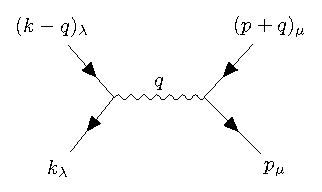
\includegraphics[width=0.7\textwidth]{feyman.pdf}
  \end{minipage}
  \begin{minipage}[c]{0.4\textwidth}
    \caption{\label{fig:4_3} Graphical representation of the potential energy term in second quantization: on the bottom we can see the effect of the two destruction operators \(  a_{p \mu } a_{k\lambda } \) which destroy particles \( k_ \lambda  \) and \( p_ \mu  \).
    Then, since we have two creation operators, as  a consequence of the Coulomb interaction \( q \), we create two particles:  \( \qty(k-q)  \) with spin \( \lambda  \)  and \( \qty(p+q)  \) with spin \( \mu  \).
    }
  \end{minipage}
\end{figure}


\end{itemize}




\subsubsection*{Total Hamiltonian}
Finally, the complete Hamiltonian of the degenerate electron gas in one dimension is the following:
\begin{equation}
  \hat{H} = \sum_{k \lambda }^{} \frac{\hbar ^2 k^2}{2m} a_{k\lambda }^\dag a_{k\lambda }
  - \frac{e^2}{2L} \sum_{\substack{k p q \\ \lambda \mu  } }^{'} \qty[  2 \qty( \gamma + \ln{\abs{q } }  ) ]
  a_{k-q, \lambda } ^\dag a_{p+q,\mu }^\dag  a_{p\mu } a_{k \lambda }
\end{equation}
where the first term corresponds to the kinetic energy term and the second one to the potential energy term where we have to remember that in the sum we should consider only \( q \neq 0 \) terms.


Essentially, our model is just characterized by two characteristic lengths:
\begin{itemize}
\item the \textbf{interparticle distance} (electron-electron), which is called \( r_0 \).

\item the \textbf{Bohr radius} \( a_0 \) is a relevant distance because the kind of interaction between electron-electron and backgorund-electrons is a Coulomb one.
\end{itemize}

The dimensionless ratio between these two lengths results:
\begin{equation*}
  r_s \equiv \frac{r_0}{a_0}
\end{equation*}

Now, since we have introduced those two parameters \( r_0,a_0 \) and this dimensionless quantity \( r_s \), we can also define other dimensionless quantities as:
\begin{equation*}
  \bar{L} \equiv \frac{L}{r_0}, \quad \bar{k} \equiv r_0 k, \quad  \bar{p} \equiv r_0 p, \quad \bar{q} \equiv r_0 q
\end{equation*}
For example:
\begin{itemize}
\item for the \emph{kinetic term}:
\begin{equation*}
  a_0 = \frac{\hbar ^2}{m e^2} \quad \rightarrow \frac{\hbar ^2}{m} = a_0 e^2
\end{equation*}
\item for the \emph{potential term}:
\begin{equation*}
  \frac{e^2}{L} \qty[  \qty( \gamma + \ln{\abs{q } }  ) ]  =
  \frac{e^2}{\bar{L}r_0} \qty[  \qty( \gamma + \ln{\abs{ \frac{\bar{q}}{r_0}  } }  ) ] =
  \frac{e^2}{\bar{L}r_s a_0} \qty[  \qty( \gamma + \ln{\abs{ \frac{\bar{q}}{r_s a_0 }  } }  ) ]
  % = \frac{e^2}{\bar{L}\bar{q}^2  }\frac{1}{r_s a_0}
  % = \qty(\frac{e^2}{2 a_0}) \frac{2}{r_s^2} \frac{r_s}{\bar{V}\bar{q}^2  }
\end{equation*}
\end{itemize}
Now, by taking into account this change in term of dimensionless variable, we can
rewrite the Hamiltonian in second quantization in this way:
\begin{equation}
  \hat{H} = \frac{e^2}{r_s^2 a_0} \qty(
  \underbrace{\sum_{k \lambda }^{} \frac{\bar{k}^2}{2} a_{k\lambda }^\dag a_{k\lambda }}_{}
  - \underbrace{\frac{r_s}{2 \bar{L} } \sum_{\substack{k p q \\ \lambda \mu  } }^{'} \qty[  2 \qty( \gamma + \ln{\abs{ \frac{\bar{q}}{r_s a_0 }  } }  ) ]
  a_{k-q, \lambda } ^\dag a_{p+q,\mu }^\dag  a_{p\mu } a_{k \lambda } }_{} ) = \hat{H}_0 + \hat{H}_1
\end{equation}


\subsection*{Perturbative approach}
The most important result is that we can rewrite schematically the Hamiltonian as the sum of \( \hat{H}_0  \)  and \( \hat{H}_1  \) contributions, where the first term is just the kinetic term and the second term is  the potential interaction term, which is multiplied by the \( r_s \) parameter. The latter, is the goal of this derivation because it implies that as \( r_s \rightarrow 0 \), the potential energy becomes a small perturbation.

Let us calculate:
\item The \textbf{unperturbate Hamiltonian} \( \mathbf{\hat{H}_0 } \).
Let us start considering
\begin{equation*}
  \hat{H}_0 = \sum_{k \lambda }^{} \frac{\hbar ^2 k^2}{2m} a_{k \lambda } ^\dag a_{k\lambda } = \sum_{k\lambda }^{} \frac{\hbar ^2 k^2}{2m} \hat{n}_{k \lambda }
\end{equation*}
that is the unperturbed Hamiltonian representing a \emph{non-interacting} Fermi system.
Now, the problem is what is our system when the particle are non interacting, the idea is simple: the system obeys the Pauli exclusion principle. Indeed, due to the Pauli exclusion principle each momentum (or wave vector) eigenstate (each single-particle state) can be occupied by only two electrons: one with spin-up and one with spin-down.
Essentially, the \emph{ground state} of the non-interacting degenerate electron gas is the so called \textbf{Fermi surface}, a surface in the momentum space (or in the reciprocal space), and the ground state is represented as \( \ket{F}  \).
In practice, the Fermi surface separates occupied from unoccupied electron states at zero temperature: inside the sphere we have all the occupied states, while outside the empty ones.
The Fermi surface is thus obtained by filling it with single-particle states up to a \emph{maximum value} (depending on the total number of particles), that is called the \textbf{Fermi momentum}:
\begin{equation*}
  p_F = \hbar k_F
\end{equation*}
that is the product of the \textbf{Fermi wave vector} per \( \hbar  \).
Clearly, the occupied states are denoted by states where:
\begin{equation*}
  \abs{k}  \le k_F
\end{equation*}
We have to respect also the boundary conditions:
\begin{equation*}
  k = \frac{2 \pi }{L}n \quad \Rightarrow   \abs{\Delta k}= \frac{2 \pi }{L}
\end{equation*}
By summing over all these states:
\begin{equation*}
  \sum_{\abs{k}  \le k_F }^{} 1 = \frac{N}{2}
\end{equation*}
this must be equal to the total number of particle divided by a factor 2, because ,due to spin degeneracy, every single state characterized by a given value of the \( k \)  wave vector can be occupied by up to two electrons (spin-up and spin-down).
Now, it is convenient to work in the thermodynamic limit \( L \rightarrow \infty  \) to replace the discrete sum with an integral over \( k \). In practice we can transform the sum into an integral as follow:
\begin{equation}
  \sum_{ k }^{}
  \overset{L \rightarrow \infty }{\rightarrow  } \frac{L}{2 \pi } \int_{}^{} \dd[]{k}
\end{equation}
In our specific case:
\begin{equation*}
  \sum_{\abs{k}  \le k_F }^{}   \overset{L \rightarrow \infty }{\rightarrow  }
  \frac{L}{2 \pi} \int_{\abs{k}  \le k_F}^{} \dd[]{k}
  = \frac{L}{2 \pi} 2 k_F = \frac{N}{2}
\end{equation*}
With such a relation we can directly relate the Fermi wave vector \( k_F \) to the particle density \( n=N/L \):
\begin{equation*}
  k_F = \frac{\pi n}{2}
\end{equation*}
Let us evaluate the 0-order term in the perturbative approach, i.e. the energy for the non-interacting system:
\begin{equation*}
  E_0 = \bra{F} \hat{H}_0 \ket{F} = \sum_{k\lambda }^{} \frac{\hbar ^2 k^2}{2m }     \bra{F} \hat{n}_{k\lambda } \ket{F}
\end{equation*}
which is just the kinetic energy contribution and it is estimated by taking the matrix element between the unperturbed ground state.
Then, we have written it in second quantization and since by its definition the effect of the number operator multiplied to a state just gives the occupation of the state itself and  since  \( \hat{n}_{k \lambda }  \) refers to the wave vector \( k \) with spin \( \lambda  \), this gives:
\begin{equation*}
  \begin{cases}
   \hat{n}_{k \lambda } \ket{F} = \ket{F} & \text{if } \abs{k} \le k_F  \\
  \hat{n}_{k \lambda } \ket{F} = 0  & \text{if } \abs{k} > k_F
  \end{cases}
\end{equation*}
with the normalization condition on the ground state \(  \braket{F}{F}=1   \).


Clearly, we can easily evaluate the matrix element in \( E_0 \):
\begin{equation*}
  E_0 = 2 \sum_{\abs{k} \le k_F }^{}  \frac{\hbar ^2 k^2}{2m}
\end{equation*}
where the 2 factor derives from the sum over the spins \( \lambda  \).
Now, we go to the thermodynamic limit:
\begin{equation}
\begin{split}
  E_0  \overset{L \rightarrow \infty }{\rightarrow } \frac{L}{2 \pi}
  2  \int_{\abs{k} \le k_F}^{} \dd[]{k} \frac{\hbar ^2 k^2}{2m}
  = \frac{L}{\pi} \frac{\hbar ^2 }{m} \frac{k_F^3}{3}
   \overset{k_F=  \frac{\pi N}{2L}}{=}
   \frac{1}{3} \underbrace{\qty(\frac{\hbar ^2 k_F^2}{2m}) }_{\varepsilon _F} N = \frac{1}{3} \varepsilon _F N
\end{split}
\end{equation}
where we have defined the \textbf{Fermi energy} as \( \varepsilon _F \).
Let us notice that:
\begin{equation*}
  \frac{E_0}{N} = \frac{1}{3} \varepsilon _F > 0
\end{equation*}
so if we compute the energy per particle, the result is positive (the Fermi energy is of order of few \( \SI{}{\eV}  \)) and in particular, even at zero temperature (remind that we implictly assume that we are working at \( T=0 \)) the total energy of the system is not zero but finite and positive.
As said, this is a consequence of the Pauli exclusion principle, because when we try to occupy the states in the Fermi sphere, with particle different from bosons, we cannot put all the electrons in the lowest energy state but we should occupy also states at finite energy.


Now, let us manipulate a little the expression of  \( k_F^2 \):
\begin{equation*}
  k_F^2 = \qty(\frac{\pi n}{2})^2 = \frac{\pi^2 }{4 r_0^2 } = \frac{\pi^2 }{4  r_s^2 a_0^2 }
\end{equation*}
Hence, the Fermi energy can be expressed as:
\begin{equation*}
  \varepsilon _F = \frac{\hbar ^2 k_F^2}{2m} = \frac{\hbar ^2}{2m} \qty(\frac{ \pi^2 }{4}) \frac{1}{r_s^2 a_0^2}
  = \qty(\frac{e^2}{2 a_0})  \mathcolorbox{yellow!40}{\underbrace{\qty(\frac{1}{e^2} \frac{\hbar ^2}{m a_0})}_{=1}  }
  \qty(\frac{\pi^2 }{4})    \frac{1}{r_s^2}
  = \qty(\frac{e^2}{2 a_0})    \qty(\frac{\pi^2 }{4})     \frac{1}{r_s^2}
\end{equation*}
where the yellow term is equal to 1 because is just the definition of the Bohr radius. Thus we can write:
\begin{equation*}
  E_0 = \frac{1}{3} \qty(\frac{e^2}{2 a_0})     \qty(\frac{\pi^2 }{4})     \frac{1}{r_s^2} N
  = 0.82 \underbrace{ \qty(\frac{e^2}{2 a_0})}_{= 1 \text{Ryd}}  \frac{1}{r_s^2} N
  = \frac{0.82}{r_s^2} N \, \text{Ryd}
\end{equation*}
where we have estimated the numerical value using the definition of Rydberg, namely the ground state energy of the Hydrogen atom.
The energy is an extensive quantity and as expected it is proportional to the number of particle \(   E_0 \sim N \).
Moreover, the energy \( E_0 \) goes as the inverse of the square of \( r_s \).

















\item The \textbf{first order correction} \( \mathbf{\hat{H}_1 } \).

In the perturbative approach, the first order correction term is obtained just by taking the matrix element of the potential energy term between the non-interacting Fermi ground state:
\begin{equation*}
  E^{(1)} = \bra{F} \hat{H}_1 \ket{F}
  =   - \frac{e^2}{2L} \sum_{\substack{k p q \\ \lambda \mu  } }^{'} \qty[  2 \qty( \gamma + \ln{\abs{q } }  ) ]
    \bra{F} a_{k-q, \lambda } ^\dag a_{p+q,\mu }^\dag  a_{p\mu } a_{k \lambda } \ket{F}
\end{equation*}
where we have
\begin{equation*}
  \begin{cases}
     a_{p \mu } a_{k \lambda } \ket{F}  \neq 0 &  \text{ only if } \abs{k} \le k_F, \abs{p} \le k_F \\
     \bra{F} a_{k - q, \lambda }^\dag a_{p+q, \mu } ^\dag = \qty(  a_{p+q, \mu } a_{k-q, \lambda } \ket{F} ) ^\dag \neq 0
     & \text{ only if } \abs{k - q} \le k_F, \abs{p + q} \le k_F
  \end{cases}
\end{equation*}
More specifically, the matrix element can be different from zero only if the two creation operators exactly fill up the holes made by the two destruction operators, namely two particles are destroyed and then two additional particles are created in exactly the same state inside the Fermi surface.







By considering the wave vector index of these operators, there are only two possibilities:
\begin{equation*}
  \begin{cases}
   k-q = k &(\lambda = \lambda )\\
   p+q = p &(\mu = \mu )
  \end{cases}
  \quad \quad \quad
  \begin{cases}
   k-q = p & (\lambda = \mu )\\
   p+q = k & (\mu = \lambda )
  \end{cases}
\end{equation*}
where the the contribution on the left is called \textbf{direct term} while the one on the right \textbf{exchange term}.

The direct term realizes only if  \( q=0 \), but  in the sum \( \sum_{}^{'}   \) the \( q=0 \) term is not considered. Hence, in our specific case, the condition in the direct term is not possible.
On the contrary, the condition of the exchange term can be realized:
\begin{equation*}
\begin{split}
  E^{(1)} &= - \frac{e^2}{2L} \sum_{\substack{k p q \\ \lambda \mu  } }^{'} \qty[  2 \qty( \gamma + \ln{\abs{q } }  ) ]
    \bra{F} a_{k-q, \lambda } ^\dag \mathcolorbox{green!20}{a_{p+q,\mu }^\dag  a_{p\mu } a_{k \lambda }} \ket{F}
   \\
   & =
   - \frac{e^2}{2L} \sum_{\substack{k p q \\ \lambda \mu  } }^{'} \qty[  2 \qty( \gamma + \ln{\abs{q } }  ) ]
     \bra{F} a_{k-q, \lambda } ^\dag \mathcolorbox{green!20}{
     \Big(-a_{k-q,\lambda  } a_{k \lambda } ^\dag  + \underbrace{\delta _{k,k-q}}_{=0\, (q \neq0)}  } \Big) a_{k \lambda} \ket{F}
\end{split}
\end{equation*}
where the green transforms due to the anticommutation rule and where the \( \delta  \) is different from zero only if \( q=0 \).  Hence, since in our case the \( q=0  \) term is not present, the \( \delta  \) gives no contribution.
By replacing the destruction and creation operator with the number ones:
\begin{equation*}
  E^{(1)} = + \frac{e^2}{2L} \sum_{\substack{k q \lambda  \\ \abs{k}\le k_F  \abs{k-q}\le k_F  } }^{'} \qty[  2 \qty( \gamma + \ln{\abs{q } }  ) ]
  \bra{F} \hat{n}_{k-q,\lambda } \hat{n}_{k \lambda } \ket{F}  >0!
\end{equation*}
this exchange term results positive.



Now, we should try to really evaluate this expression. First of all, we observe that:
\begin{equation*}
  \begin{cases}
  \hat{n}_{k \lambda } =\ket{F} & \text{if } \abs{k}\le k_F   \\
  \hat{n}_{k-q, \lambda } =\ket{F} & \text{if } \abs{k-q}\le k_F
  \end{cases}
\end{equation*}
Therefore, we get:
\begin{equation*}
\begin{split}
  E^{(1)} &= +\frac{e^2}{2L} \sum_{\substack{k q \lambda  \\ \abs{k}\le k_F  \abs{k-q}\le k_F  } }^{'} \qty[  2 \qty( \gamma + \ln{\abs{q } }  ) ] \\
  &\underset{L \rightarrow \infty }{\longrightarrow }
  + \frac{\mathcolorbox{yellow!40}{2}e^2}{2L} \frac{L^2}{(2 \pi )^2}
  \int_{}^{} \dd[]{k}
  \int_{}^{} \dd[]{q} \qty[  2 \qty( \gamma + \ln{\abs{q } }  ) ]
  \Theta (k_F- k) \Theta (k_F - \abs{k-q} ) \\
\end{split}
\end{equation*}
where by considering the thermodynamic limit we compute integrals instead of sums (it is simpler), going from a double sum to a double integral. In particular, we get the yellow term "2" by summing over \( \lambda  \) and  the \( \theta  \) functions are introduced to enforce the conditions in the sums. Moreover, \( q \neq 0 \) can be omitted since it effects the integrand at only a single point, so it is negligible compared to the rest of the contribution.







Now it is convenient to make the expression more symmetric. For that purpose, we introduce new variables:
\begin{equation*}
  p \equiv k - \frac{q}{2} \quad \Rightarrow k = p+\frac{q}{2}
\end{equation*}
Thus we obtain:
\begin{equation*}
  E^{(1)} = + \frac{ e^2 L}{2 \pi^2}
  \int_{}^{} \dd[]{q} \qty[   \qty( \gamma + \ln{\abs{q } }  ) ]
  \int_{}^{} \dd[]{p} \Theta \qty(k_F - \abs{ p+\frac{q}{2} } )
  \Theta \qty(k_F - \abs{p-\frac{q}{2} } )
\end{equation*}
and considering that \( \abs{p\pm\frac{q}{2}} \le k_F \), the region of integration over \( p \) is the intersection between 2 line segment of length \(2 k_F \). Indeed, you can have a non vanishing contribution only if \( \abs{q } \le 2 k_F  \).
\begin{equation*}
  E^{(1)} = + \frac{ e^2 L}{2 \pi^2}
  \int_{}^{} \dd[]{q} \qty[   \qty( \gamma + \ln{\abs{q } }  ) ]
  \qty(2k_F- \abs{q} )
  \Theta \qty(2 k_F - \abs{q}  )
\end{equation*}
It is convenient to go to dimensionless variables:
\begin{equation*}
  x \equiv \frac{q}{2k_F}, \quad \hat{\gamma  } = \gamma  + \ln{2k_F}
\end{equation*}
Hence:
\begin{equation}
\begin{split}
  E^{(1)} &= + \frac{ e^2 L}{2 \pi^2} 4 k_F^2
  \int_{}^{} \dd[]{x} \qty[   \qty( \hat{\gamma  }  + \ln{\abs{ x } }  ) ]
  \qty(1- \abs{x} )
  \Theta \qty(1- \abs{x} ) \\
  &=\frac{ e^2 L}{2 \pi^2} 4 k_F^2
  \int_{0}^{1} \dd[]{x} \qty[   \qty( \hat{\gamma  }  + \ln{\abs{ x } }  ) ]
  \qty(1- \abs{x} ) \\
  &= \frac{ e^2 L}{2 \pi^2} 4 k_F^2 \frac{1}{4} (-3 + 4 \hat{\gamma  } ) =
  \frac{ e^2 L}{2 \pi^2} 4 k_F^2 \frac{1}{4} (-3 + 4 \gamma  + 4\ln{(2k_F)} ) \\
  & \overset{k_F = \frac{\pi}{2 r_s a_0}}{=}
   \frac{ e^2 L}{2 \pi^2} 4 \qty(\frac{\pi ^2}{4 r_s^2 a_0^2} )  \frac{1}{4} (-3 + 4 \gamma  + 4\ln{\frac{2 \pi}{2 r_s a_0}} ) \\
   &=
   \frac{ e^2 L}{2 \pi^2} 4 \qty(\frac{\pi ^2}{4 r_s^2 a_0^2} )  \frac{1}{4} (-3 + 4 \gamma  + 4\ln{\frac{ \pi}{ a_0}}  - 4 \mathcolorbox{red!40}{\ln{r_s}} )
\end{split}
\end{equation}
which diverges since we have a logarithmic divergence in \( r_s\) in the limit \(r_s \rightarrow 0 \) (red term).


















\end{itemize}










\end{document}
